\chapter{Fundamentals} \label{chap:fundamentos}
In this chapter, we will explore the fundamental concepts used throughout this work, including Neural Networks, Quantization, Adversarial Attack, and Neural Network Robustness Verification.

%--------------------------------------------
\section{Artificial Neural Networks}
\label{sec:nn}
%--------------------------------------------

ANNs are a class of machine learning models inspired by the structure and function of the human brain \cite{mcculloch1943logical}. The correlation with the human brain was drawn because it consists of interconnected nodes, such as neurons, arranged in layers that collectively transform input data into output predictions. The primary appeal lies in their ability to approximate highly non-linear functions and automatically learn relevant features from raw data \cite{goodfellow2016deep}.

The origins of neural networks trace back to the seminal work that introduced a simplified mathematical model of a neuron \cite{mcculloch1943logical}. This was followed by Rosenblatt's Perceptron \cite{Rosenblatt1958}, which could learn linear decision boundaries but was shown to be incapable of solving linearly inseparable problems, such as the XOR classification task~\cite{minsky1969perceptrons}. This limitation, widely publicized in~\cite{minsky1969perceptrons}, contributed to reduced research interest during the so-called ``AI Winter.'' The revival came in the 1980s with the formalization and popularization of the \textit{backpropagation} algorithm \cite{werbos1974beyond,rumelhart1986learning}, which enabled the efficient training of multi-layer perceptrons (MLPs) and, later, deep neural networks (DNNs).

In its modern form, a neural network is organized into an input layer, one or more hidden layers, and an output layer, with each layer $l \in \{1, \dots, L\}$ containing a set of neurons that together construct the entire network architecture.

The basic operation of a layer can be expressed as:
%\begin{equation}
%    y = f\left( \sum_{i=1}^{n} w_i x_i + b \right),
%    \end{equation}
\begin{equation}
y = f\left(\sum_{i=1}^{n} w_i x_i + b\right)
\end{equation}

where $x_i$ are the inputs, $w_i$ the corresponding weights, $b$ a bias term, and $f(\cdot)$ a non-linear activation function. The linear operation $w_i x_i + b$ within the activation function $f(\cdot)$ can be considered a layer itself, called an affine layer.

The most common activation functions include sigmoid, ReLU (Rectified Linear Unit), and tanh (hyperbolic tangent). The sigmoid function maps inputs to a range between 0 and 1; The ReLu function outputs the input directly if it is positive; otherwise, it outputs zero; lastly, the tanh function maps inputs to a range between -1 and 1. These functions introduce non-linearity into the model, allowing it to learn complex relationships in the data.

Figure \ref{fig:activation_function} illustrates examples of these activation functions.


\begin{figure}[!ht]
    \centering
    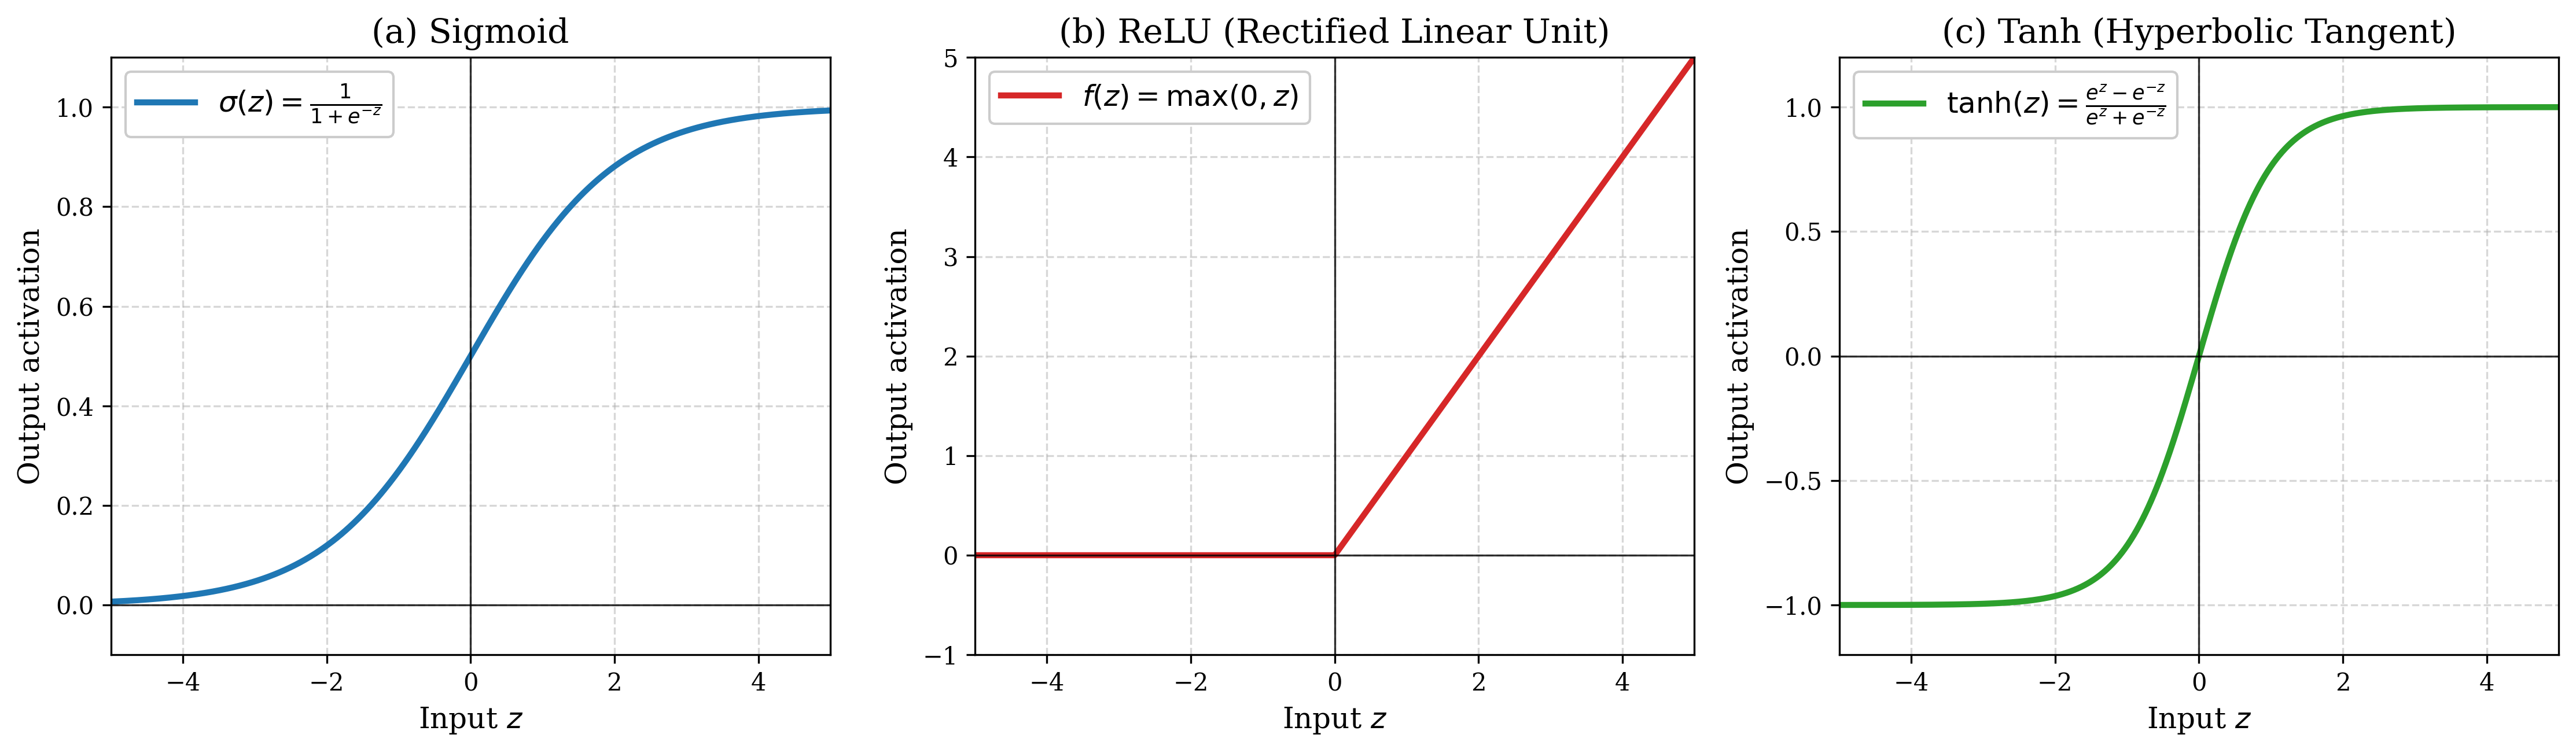
\includegraphics[width=1\textwidth]{figuras/2-fundamentos/activation_functions_combined.png}
    \caption{Activation Functions Examples: Sigmoid, ReLU, and Tanh}
    \label{fig:activation_function}
    \end{figure}

These neurons are the core components of various neural network architectures, which can be organized into layers; the input layer receives the initial data, hidden layers process the data through multiple transformations, and the output layer produces the final predictions or classifications, as shown in Figure \ref{fig:neural_network_architecture}. 
\newpage
\begin{figure}[!ht]
    \centering
    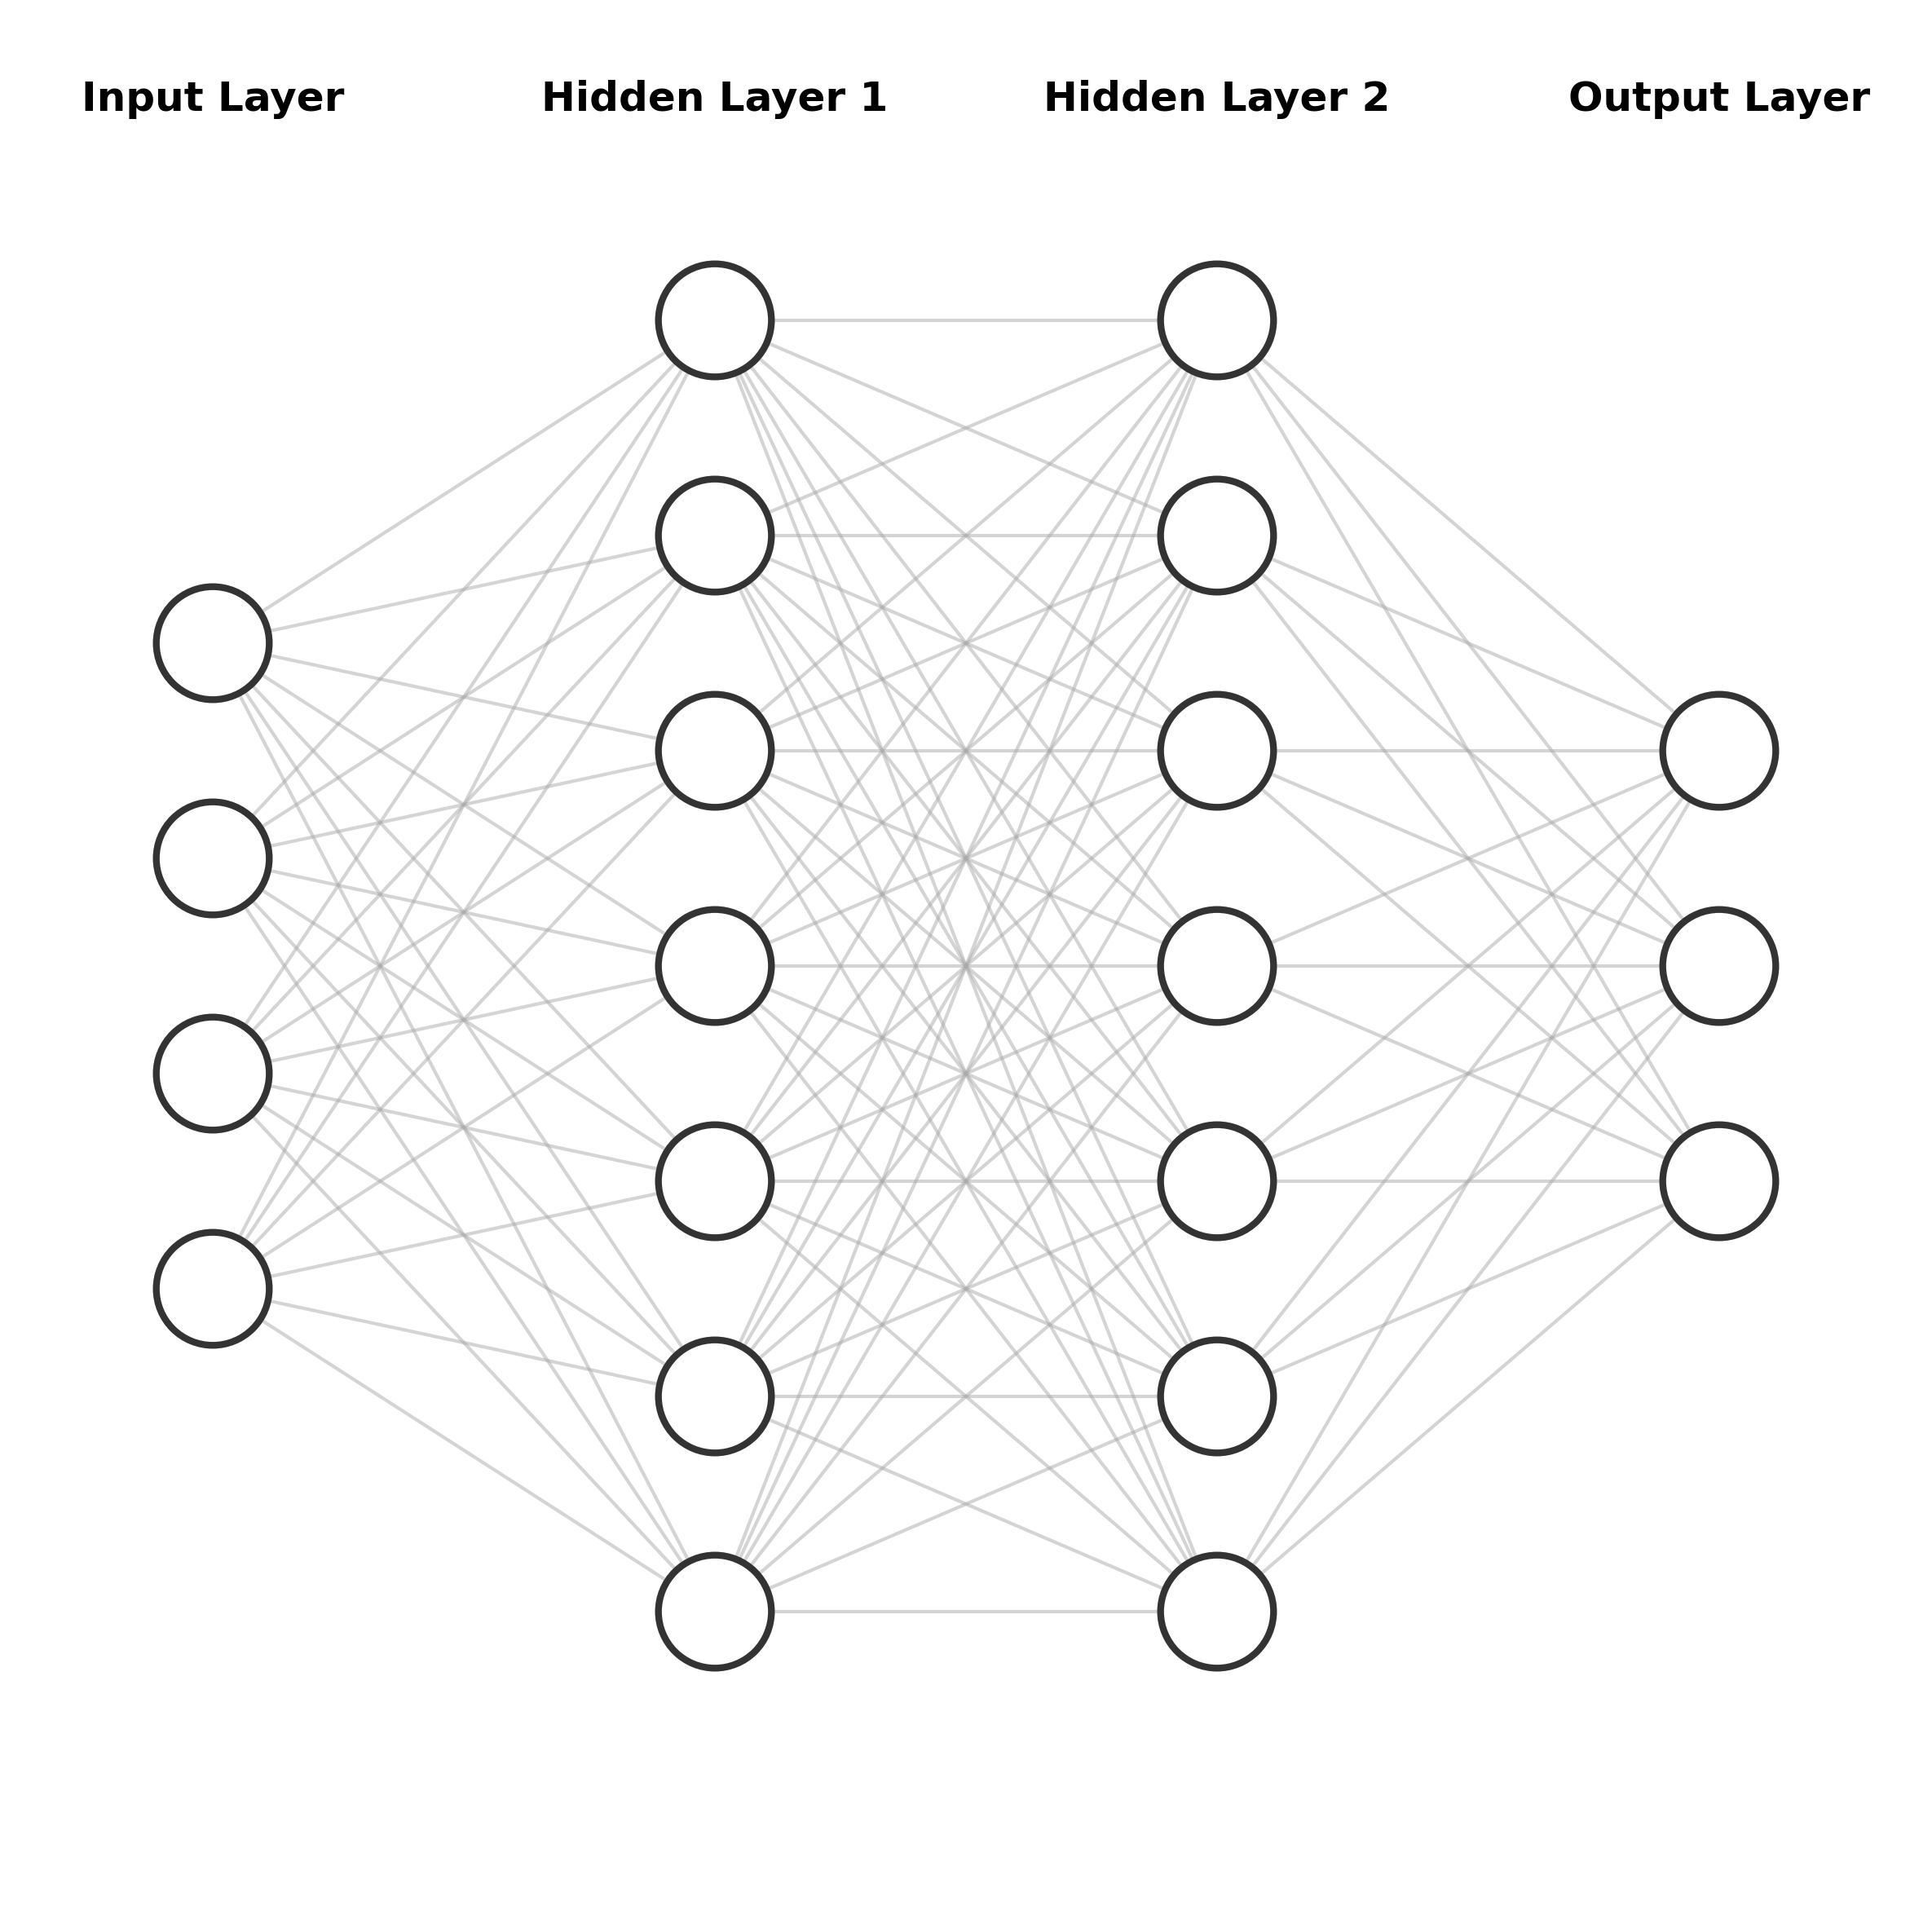
\includegraphics[width=1\textwidth]{figuras/2-fundamentos/neural_network_diagram.png}
    \caption{Diagram of a Neural Network with Input, Hidden, and Output Layers \cite{duda2001pattern}}
    \label{fig:neural_network_architecture}
    \end{figure}

  In practice, it is more convenient to express the forward computation of an entire layer using vectorized notation:
  %  \begin{align}
  %      \mathbf{z}^{[l]} &= \mathbf{W}^{[l]} \mathbf{a}^{[l-1]} + \mathbf{b}^{[l]}, \\
  %      \mathbf{a}^{[l]} &= \sigma^{[l]}\left( \mathbf{z}^{[l]} \right),
  %      \end{align}
\begin{align}
\mathbf{z}^{[l]} = \mathbf{W}^{[l]} \mathbf{a}^{[l-1]} + \mathbf{b}^{[l]}\\
\mathbf{a}^{[l]} = \mathbf{\sigma}^{[l]}(\mathbf{z}^{[l]})
\end{align}

\noindent where $\mathbf{a}^{[0]} = \mathbf{x}$ denotes the input vector, $\mathbf{W}^{[l]} \in \mathbb{R}^{n_l \times n_{l-1}}$ is the weight matrix, $\mathbf{b}^{[l]} \in \mathbb{R}^{n_l}$ is the bias vector, and $\sigma^{[l]}(\cdot)$ is the activation function applied element-wise.
\begin{comment}
    
\begin{figure}[H]
    \centering
    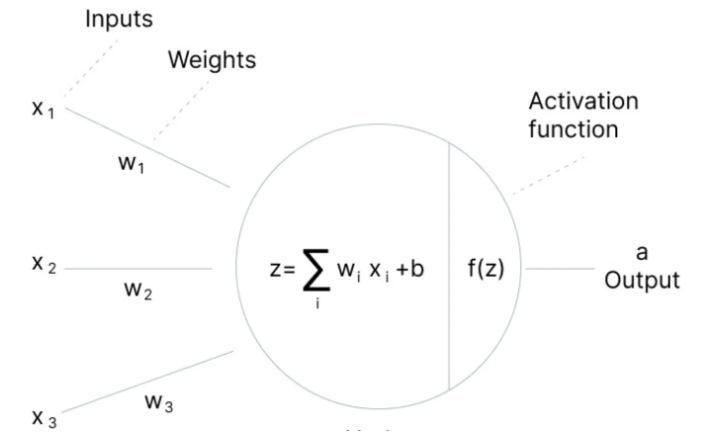
\includegraphics[width=0.8\textwidth]{figuras/2-fundamentos/neural_node.png}
    \caption{Schematic of an artificial neuron: inputs $x_i$ are weighted by $w_i$, summed with a bias $b$, and passed through a non-linear activation function $f(\cdot)$ to produce the output $y$.}
    \label{fig:neuron_diagram}
\end{figure}
\end{comment}

For supervised learning tasks, the output of the final layer $\mathbf{a}^{[L]}$ is compared with the target $\mathbf{y}$ via a differentiable loss function $\mathcal{L}(\mathbf{a}^{[L]}, \mathbf{y})$. The objective of training is to minimize the cost function:
\begin{equation}
    %J(\mathbf{W}, \mathbf{b}) = \frac{1}{m} \sum_{i=1}^m \mathcal{L}\big( \mathbf{a}^{[L](i)}, \mathbf{y}^{(i)} \big),
J(\mathbf{W}, \mathbf{b}) = \frac{1}{m} \sum_{i=1}^{m} \mathcal{L}(\mathbf{a}^{[L](i)}, \mathbf{y}^{(i)})
\end{equation}
\noindent where $m$ is the number of training samples. This minimization requires computing the gradients of $J$ with respect to each parameter $\mathbf{W}^{[l]}$ and $\mathbf{b}^{[l]}$. 

Computing these gradients is expensive due to the network's layered structure. The breakthrough of the backpropagation algorithm \cite{rumelhart1986learning} was to systematically exploit the chain rule of calculus, allowing gradients to be propagated efficiently from the output layer back through the hidden layers. This efficiency reduced the computational cost to a scale proportional to that of the forward pass, making it feasible to train networks with many layers and large numbers of parameters.

Today, neural networks form the foundation of deep learning systems used in various domains such as computer vision \cite{lecun1998gradient}, natural language processing \cite{vaswani2017attention}, and embedded AI for robotics and IoT \cite{lane2017squeezing}. Their adaptability across architectures, from convolutional neural networks (CNNs) to transformers, underscores the enduring relevance of the concepts introduced more than four decades ago.
%\textcolor{red}{this sentence uses the same style of ChatGPT :-) Please check if your text does not contain AI-written patterns} \textcolor{blue}{fixed}.


\begin{comment}
\subsection{Neural Network Architecture}

The architecture of a neural network is composed of layers of interconnected neurons. Each neuron receives inputs, applies a weighted sum followed by an activation function, and produces an output that is passed to the next layer of neurons. 

The basic building block of a neural network is the artificial neuron, which can be mathematically represented as follows:

\begin{equation}
    y = f\left(\sum_{i=1}^{n} w_i x_i + b\right)
    \end{equation}
    
    where \(y\) is the output, \(w_i\) are the weights, \(x_i\) are the inputs, \(b\) is the bias, and \(f\) is the activation function. The activation function introduces non-linearity into the model, allowing it to learn complex relationships in the data.
    
    Or visually as shown in Figure \ref{fig:neuron_diagram}, where the inputs are multiplied by their corresponding weights, summed up, and then passed through an activation function to produce the output.
    
    \newpage
    
    \begin{figure}
    \centering
    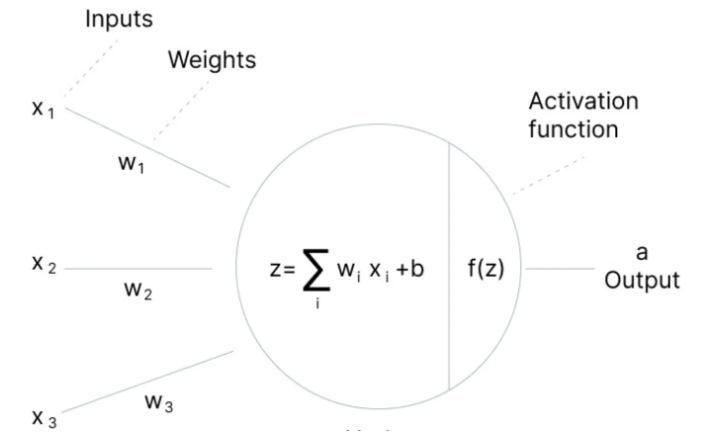
\includegraphics[width=0.8\textwidth]{figuras/2-fundamentos/neural_node.png}
    \caption{Diagram of a Single Neuron \cite{neural_node_pic}}
    
    \label{fig:neuron_diagram}
    \end{figure}
    
    Neural networks can be organized into various topologies, with the most common being Feedforward Neural Networks (FNN) and Multi-Layer Perceptrons (MLP)\cite{goodfellow2016deep}. FNNs consist of an input layer, one or more hidden layers, and an output layer, where information flows in one direction. MLPs are a specific type of FNN that includes multiple layers of neurons, allowing for more complex representations.
    
    Convolutional Neural Networks (CNNs) are another important architecture, particularly in computer vision tasks. They utilize convolutional layers to automatically learn spatial hierarchies of features from images, making them highly effective for image classification and object detection.
    
    
    % 3. Training Process
    % 3.1. Supervised Learning
    % Concept of labeled data

% Dataset split (training, validation, test)

% 3.2. Loss Functions
% MSE, Cross-Entropy (brief mention)

% 3.3. Optimization
% Gradient descent and variants (SGD, Adam)
\subsection{Training Process}
The training process of neural networks typically involves supervised learning, where the model learns from labeled data. The dataset is usually split into three parts: training, validation, and test sets. The training set is used to train the model, the validation set helps tune parameters, and the test set evaluates the model's performance on unseen data.

Loss functions are crucial in training, as they quantify the difference between the predicted outputs and the actual
labels. Common loss functions include Mean Squared Error (MSE) for regression tasks and Cross-Entropy for classification tasks shown respectively in Equations \ref{eq:mse} and \ref{eq:cross_entropy}. The choice of loss function depends on the specific task and the nature of the data.

\begin{equation}\label{eq:mse}
    \frac{1}{n} \sum_{i=1}^{n} (y_i - \hat{y}_i)^2
\end{equation}

\begin{equation}\label{eq:cross_entropy}
    -\sum_{i=1}^{n} y_i \log(\hat{y}_i)
\end{equation}

% 3.4. Backpropagation Algorithm
% How the backpropagation algorithm works
% Gradient calculation and weight updates
% Importance of backpropagation in training neural networks

These loss functions are used within backpropagation algorithm, which is the core of the training process.


% Backpropagation algorithm (brief overview or diagram)

% 4. Inference Process
% What happens when the model is deployed

% Importance of performance, size, and speed (hinting at quantization need)

% How a trained model maps input -> output

\subsubsection*{Backpropagation}
Backpropagation, short for \textit{backward propagation of errors}, is the fundamental algorithm for training artificial neural networks, enabling the efficient computation of gradients of a loss function with respect to the network’s parameters \cite{rumelhart1986learning}. It leverages the chain rule of calculus to propagate errors from the output layer back to earlier layers, systematically adjusting the weights and biases to minimize prediction error. The method was popularized in the mid-1980s, although its theoretical underpinnings can be traced back to earlier works in control theory and automatic differentiation \cite{werbos1974beyond}. Today, it remains the backbone of most supervised deep learning frameworks, being used in conjunction with optimizers such as stochastic gradient descent (SGD) and Adam.

The process begins with a \emph{forward pass}, in which the input vector $x \in \mathbb{R}^{n_0}$ is propagated layer by layer through the network. For a feedforward architecture with $L$ layers, each layer $l \in \{1, \dots, L\}$ computes a pre-activation vector $z^{[l]}$ and an activation vector $a^{[l]}$ according to
\begin{equation}
z^{[l]} = W^{[l]} a^{[l-1]} + b^{[l]}, \quad a^{[l]} = \sigma^{[l]}(z^{[l]}),
\end{equation}
where $W^{[l]} \in \mathbb{R}^{n_l \times n_{l-1}}$ is the weight matrix, $b^{[l]} \in \mathbb{R}^{n_l}$ is the bias vector, and $\sigma^{[l]}(\cdot)$ is a differentiable activation function such as the sigmoid, hyperbolic tangent, or ReLU. The input layer is given by $a^{[0]} = x$, and the network output is $\hat{y} = a^{[L]}$. The discrepancy between $\hat{y}$ and the target $y$ is measured by a differentiable loss function $\mathcal{L}(\hat{y}, y)$, and the cost over a batch of $m$ samples is
\begin{equation}
    J(W,b) = \frac{1}{m} \sum_{i=1}^{m} \mathcal{L}\big(a^{[L](i)}, y^{(i)}\big).
\end{equation}

Once the forward pass has produced the output, the \emph{backward pass} applies the chain rule to determine how a small change in each parameter affects the loss. At the output layer, the error signal is computed as
\begin{equation}
\delta^{[L]} = \nabla_a \mathcal{L}\big(a^{[L]}, y\big) \odot \sigma'^{[L]}\big(z^{[L]}\big),
\end{equation}
where $\odot$ denotes elementwise multiplication. For each preceding hidden layer $l = L-1, \dots, 1$, the error term is propagated backwards as
\begin{equation}
\delta^{[l]} = \big(W^{[l+1]}\big)^{T} \delta^{[l+1]} \odot \sigma'^{[l]}\big(z^{[l]}\big),
\end{equation}
effectively applying the chain rule to relate the sensitivity of the cost to parameters in earlier layers. Given these $\delta$ terms, the gradients with respect to the parameters are
\begin{align}
\frac{\partial J}{\partial W^{[l]}} &= \frac{1}{m} \delta^{[l]} \big(a^{[l-1]}\big)^{T}, \\
\frac{\partial J}{\partial b^{[l]}} &= \frac{1}{m} \sum_{i=1}^m \delta^{[l](i)}.
\end{align}
Finally, the parameters are updated via gradient descent,
\begin{align}
W^{[l]} &\gets W^{[l]} - \eta \frac{\partial J}{\partial W^{[l]}}, \\
b^{[l]} &\gets b^{[l]} - \eta \frac{\partial J}{\partial b^{[l]}},
\end{align}
where $\eta > 0$ is the learning rate.

The efficiency of backpropagation arises from its reuse of intermediate computations from the forward pass, avoiding redundant derivative calculations. In fact, its computational complexity is $\mathcal{O}(n)$ in the number of parameters, making it feasible for networks with millions of weights. This property, combined with the ability to use vectorized matrix operations, has made it the method of choice for modern GPUs and TPUs \cite{goodfellow2016deep}.

A high-level pseudocode for the algorithm is shown in Algorithm~\ref{alg:backprop}, where the vectorized formulation is used for batch processing. An illustration of the flow of information during forward and backward passes is provided in Figure~\ref{fig:backprop_flow}, which should be replaced with a network diagram showing activations $a^{[l]}$, pre-activations $z^{[l]}$, and gradients $\delta^{[l]}$.

\begin{figure}[H]
\centering
\includegraphics[width=0.85\linewidth]{figuras/2-fundamentos/backpropagation_flow.png}
\caption{Placeholder: Forward (left) and backward (right) propagation in a feedforward neural network \cite{duda2001pattern}}
\label{fig:backprop_flow}
\end{figure}

\begin{algorithm}[H]
\caption{Vectorized Backpropagation for a Fully Connected Neural Network}
\label{alg:backprop}
\begin{algorithmic}[1]
\Require Training data $\{(x^{(i)}, y^{(i)})\}_{i=1}^m$, learning rate $\eta$, number of layers $L$
\State Initialize $W^{[l]}, b^{[l]}$ for $l = 1, \dots, L$
\While{stopping criterion not met}
\State \textbf{Forward Pass:}
\State $A^{[0]} \gets X$
\For{$l = 1$ to $L$}
\State $Z^{[l]} \gets W^{[l]} A^{[l-1]} + b^{[l]}$
\State $A^{[l]} \gets \sigma^{[l]}(Z^{[l]})$
\EndFor
\State Compute cost $J$
\State \textbf{Backward Pass:}
\State $\Delta^{[L]} \gets \nabla_A \mathcal{L}(A^{[L]}, Y) \odot \sigma'^{[L]}(Z^{[L]})$
\For{$l = L-1$ down to $1$}
\State $\Delta^{[l]} \gets (W^{[l+1]})^T \Delta^{[l+1]} \odot \sigma'^{[l]}(Z^{[l]})$
\EndFor
\State \textbf{Parameter Updates:}
\For{$l = 1$ to $L$}
\State $W^{[l]} \gets W^{[l]} - \eta \frac{1}{m} \Delta^{[l]} (A^{[l-1]})^T$
\State $b^{[l]} \gets b^{[l]} - \eta \frac{1}{m} \sum_{i=1}^m \Delta^{[l](i)}$
\EndFor
\EndWhile
\end{algorithmic}
\end{algorithm}

From a theoretical standpoint, backpropagation can be interpreted as a special case of reverse-mode automatic differentiation, optimized for layered computational graphs. It assumes differentiable activation functions and loss functions, and its performance may degrade in very deep networks due to the vanishing and exploding gradient problems \cite{hochreiter1998vanishing}. Solutions such as careful weight initialization, normalization layers, and activation function design (e.g., ReLU, Leaky ReLU, GELU) have been developed to mitigate these issues.

In conclusion, backpropagation is the mathematical and computational framework that enables neural networks to learn from data by efficiently computing gradients through the chain rule. Its elegance lies in its generality: once the forward computation of a network is defined, the backward computation follows mechanically, allowing it to adapt seamlessly to a wide range of architectures, from simple perceptrons to modern transformers \cite{goodfellow2016deep}.

\end{comment}

During inference, the trained model is used to predict from input data. The performance, size, and speed of the model are critical factors in this process, especially in resource-constrained environments such as embedded systems and edge devices. The trained model maps input data to output predictions by applying the learned weights and biases through the network's layers.


% 5. Challenges and Motivations for Compression
% Overparameterization

% Memory usage

% Latency

% Deployment on microcontrollers, edge devices

\subsection{Challenges and Motivations for Compression}
Despite their effectiveness, ANNs face several challenges, especially Overparameterization, which can lead to significant increases in memory usage and inference latency \cite{han2016deep}. These challenges become particularly pronounced when deploying embedded systems models, where resources are limited. One standard solution to these challenges is quantization, which reduces model precision to enable faster inference and lower memory usage. 

\section{Quantization}

%1.1 Definition and Basic Idea
%General concept: reducing the precision of data by mapping continuous or high-precision values to a smaller set of fixed levels.

Quantization is a model compression technique that reduces the numerical precision of neural network parameters and activations, thereby lowering both memory usage and computational costs \cite{jacob2018quantization,han2016deep}. In summary, the idea is to map floating-point precision values to smaller, discrete fixed-precision ones. It’s by far one of the most widely used methods to make neural network computations less resource-intensive and has been proven effective for deploying ANN models on low-end devices, e.g., embedded hardware.

Mathematically, given a real-valued matrix of activations or weights $\mathbf{A} \in \mathbb{R}^{m \times p}$ and a target bit-width $n$, the quantization operator $Q$ can be defined as:
\begin{equation}
%Q(n, \mathbf{A}) = \text{clip}\left( \text{round}\left(\frac{\mathbf{A}}{q(\mathbf{A}, n)}\right)-Z,\ -2^{n-1},\ 2^{n-1}-1 \right),
Q(\mathbf{A}, n, \alpha, \beta) = \text{clip}\left(\left\lfloor \frac{\mathbf{A} - \alpha}{\frac{\beta - \alpha}{2^n - 1}} \right\rceil, 0, 2^n-1\right)\\
\label{eq:quantization}
\end{equation}
where $q(\mathbf{A}, n)$ is the scaling factor, $\text{round}(\cdot)$ rounds to the nearest integer, $\text{clip}(\cdot)$ restricts values to the range $[-2^{n-1}, 2^{n-1}-1]$ and $Z$ is an integer zero point.

The scaling factor $q(\mathbf{A}, n)$ partitions the dynamic range of $\mathbf{A}$ into $2^n$ equally spaced levels:
\begin{equation}
%q(\mathbf{A}, n) = \frac{\beta - \alpha}{2^n - 1},
q(\mathbf{A}, n) = \frac{\beta - \alpha}{2^n - 1},
\label{eq:scaling}
\end{equation}
where $\alpha = \min(\mathbf{A})$ and $\beta = \max(\mathbf{A})$. The dequantization step reconstructs an approximation $\hat{\mathbf{A}}$ of the original values:
\begin{equation}
\hat{\mathbf{A}} = q(\mathbf{A}, n) \cdot Q(n, \mathbf{A}).
\label{eq:dequantization}
\end{equation}

Figures~\ref{fig:quant_n1} and \ref{fig:quant_n2} illustrate uniform quantization for $n=1$ and $n=2$, respectively, showing the effect of reducing the representable precision.
\begin{figure}[!ht]
    \centering
    \begin{minipage}{0.8\textwidth}
        \centering
        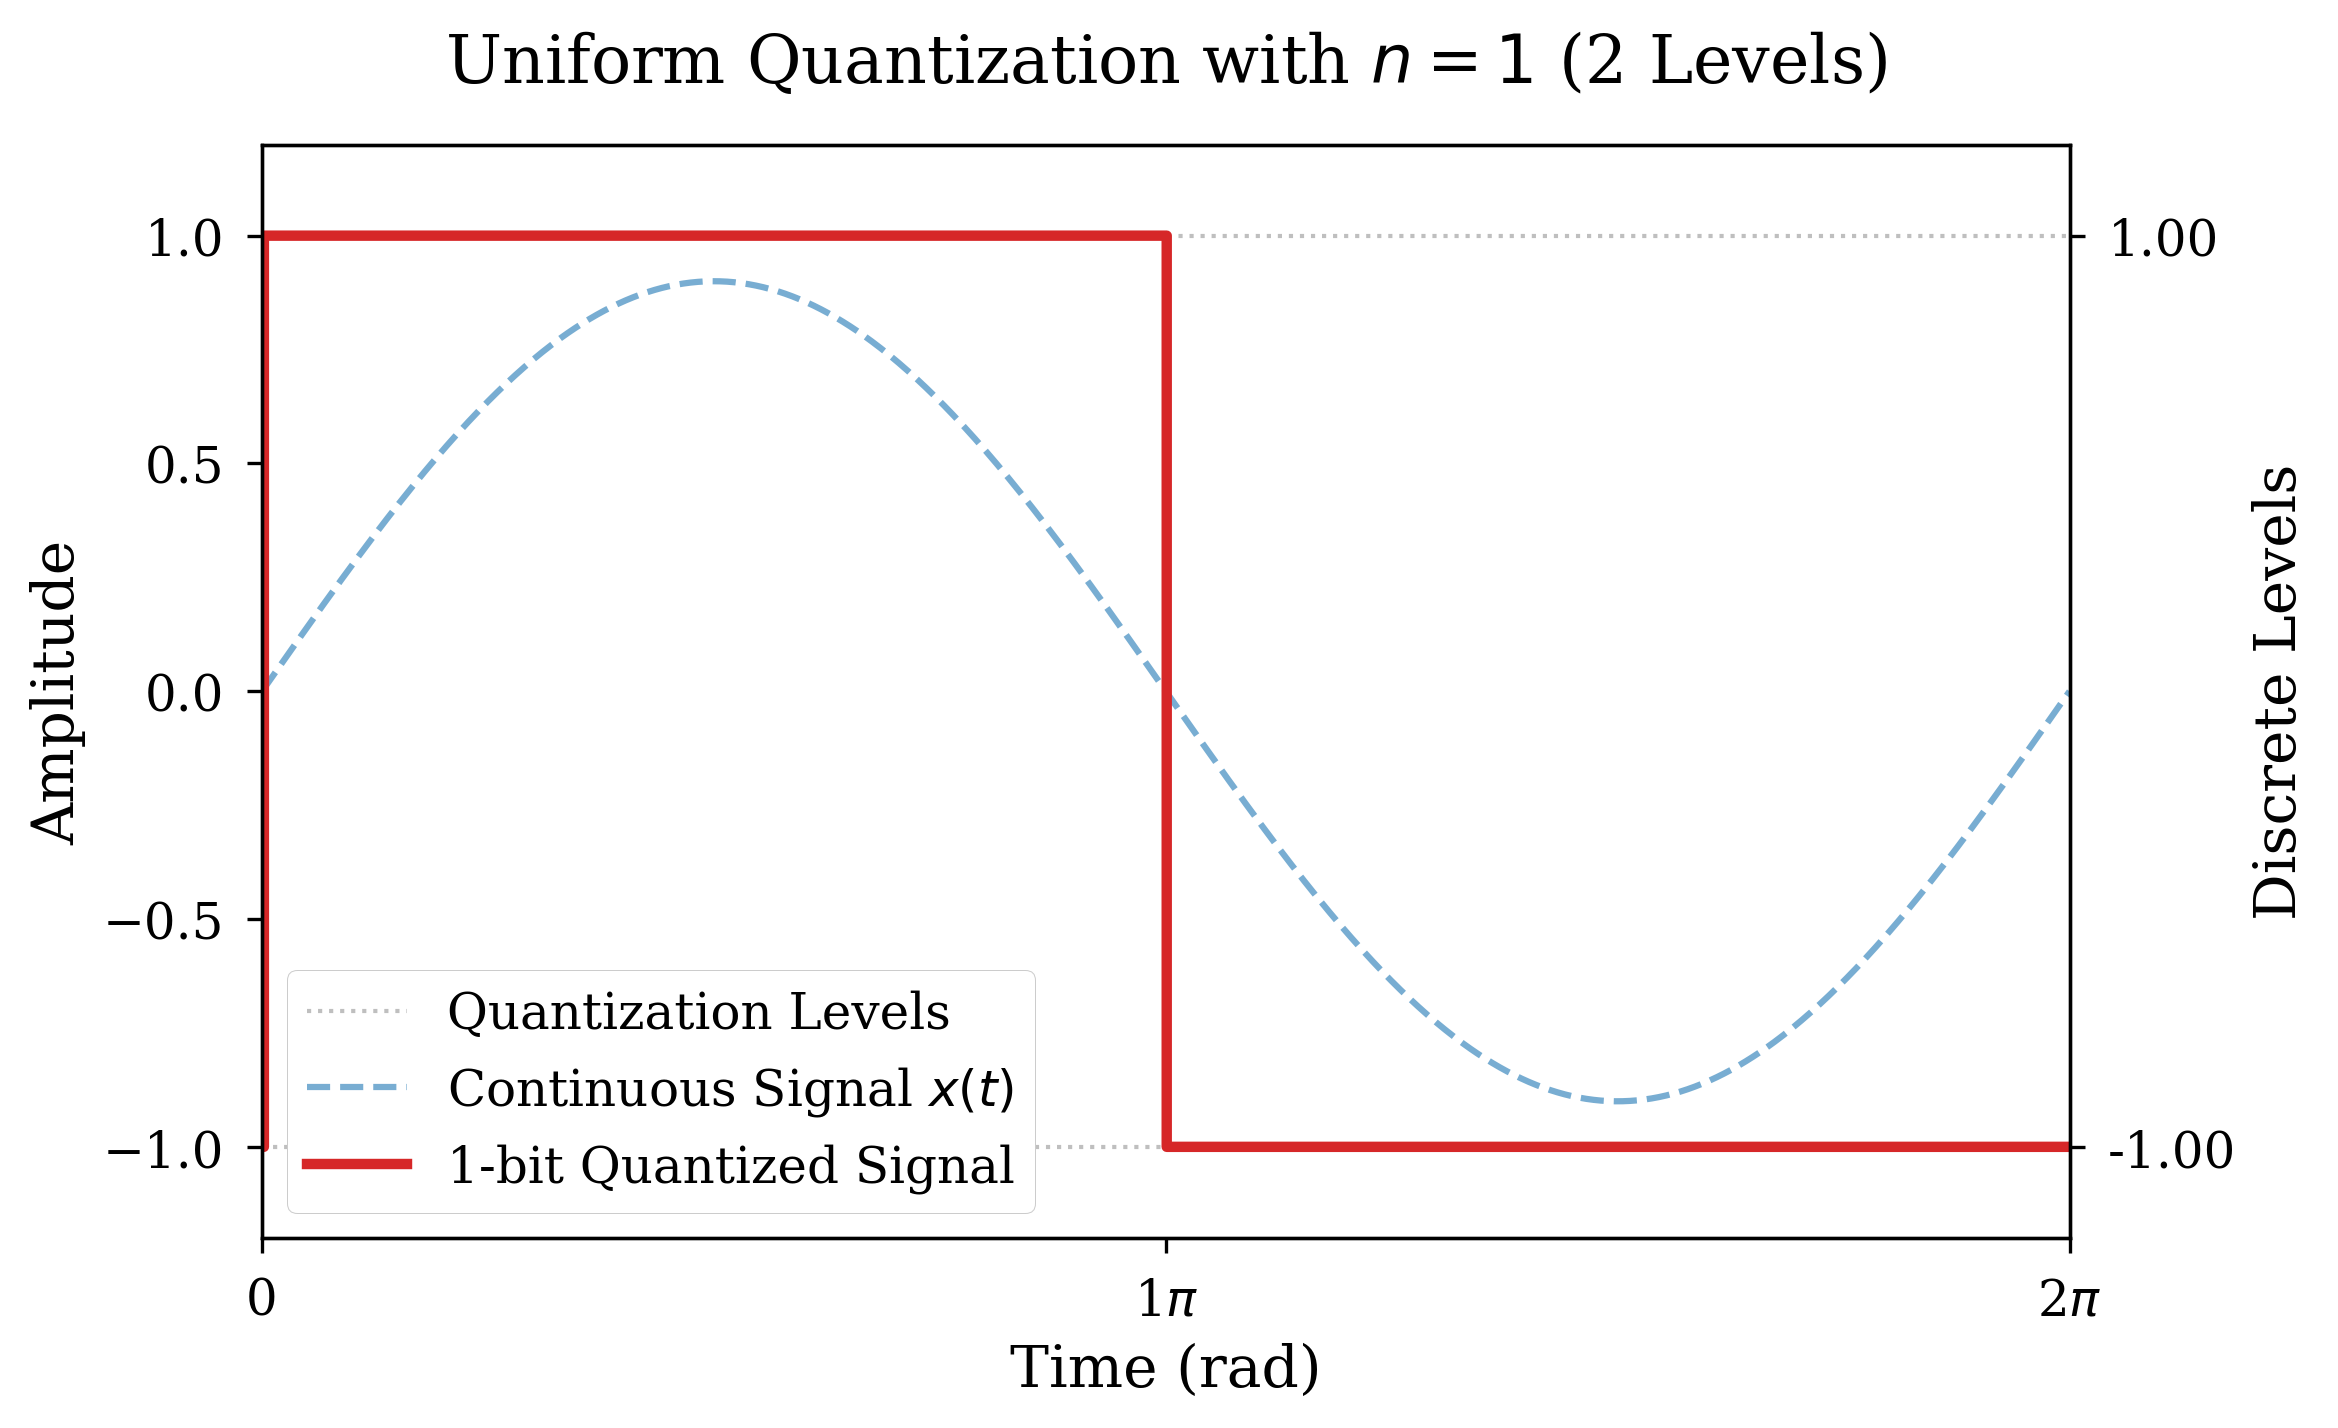
\includegraphics[width=0.75\linewidth]{figuras/2-fundamentos/quantization_n_1.png}
        \caption{Uniform quantization with $n=1$.}
        \label{fig:quant_n1}
    \end{minipage}
    \hfill
    \begin{minipage}{0.8\textwidth}
        \centering
        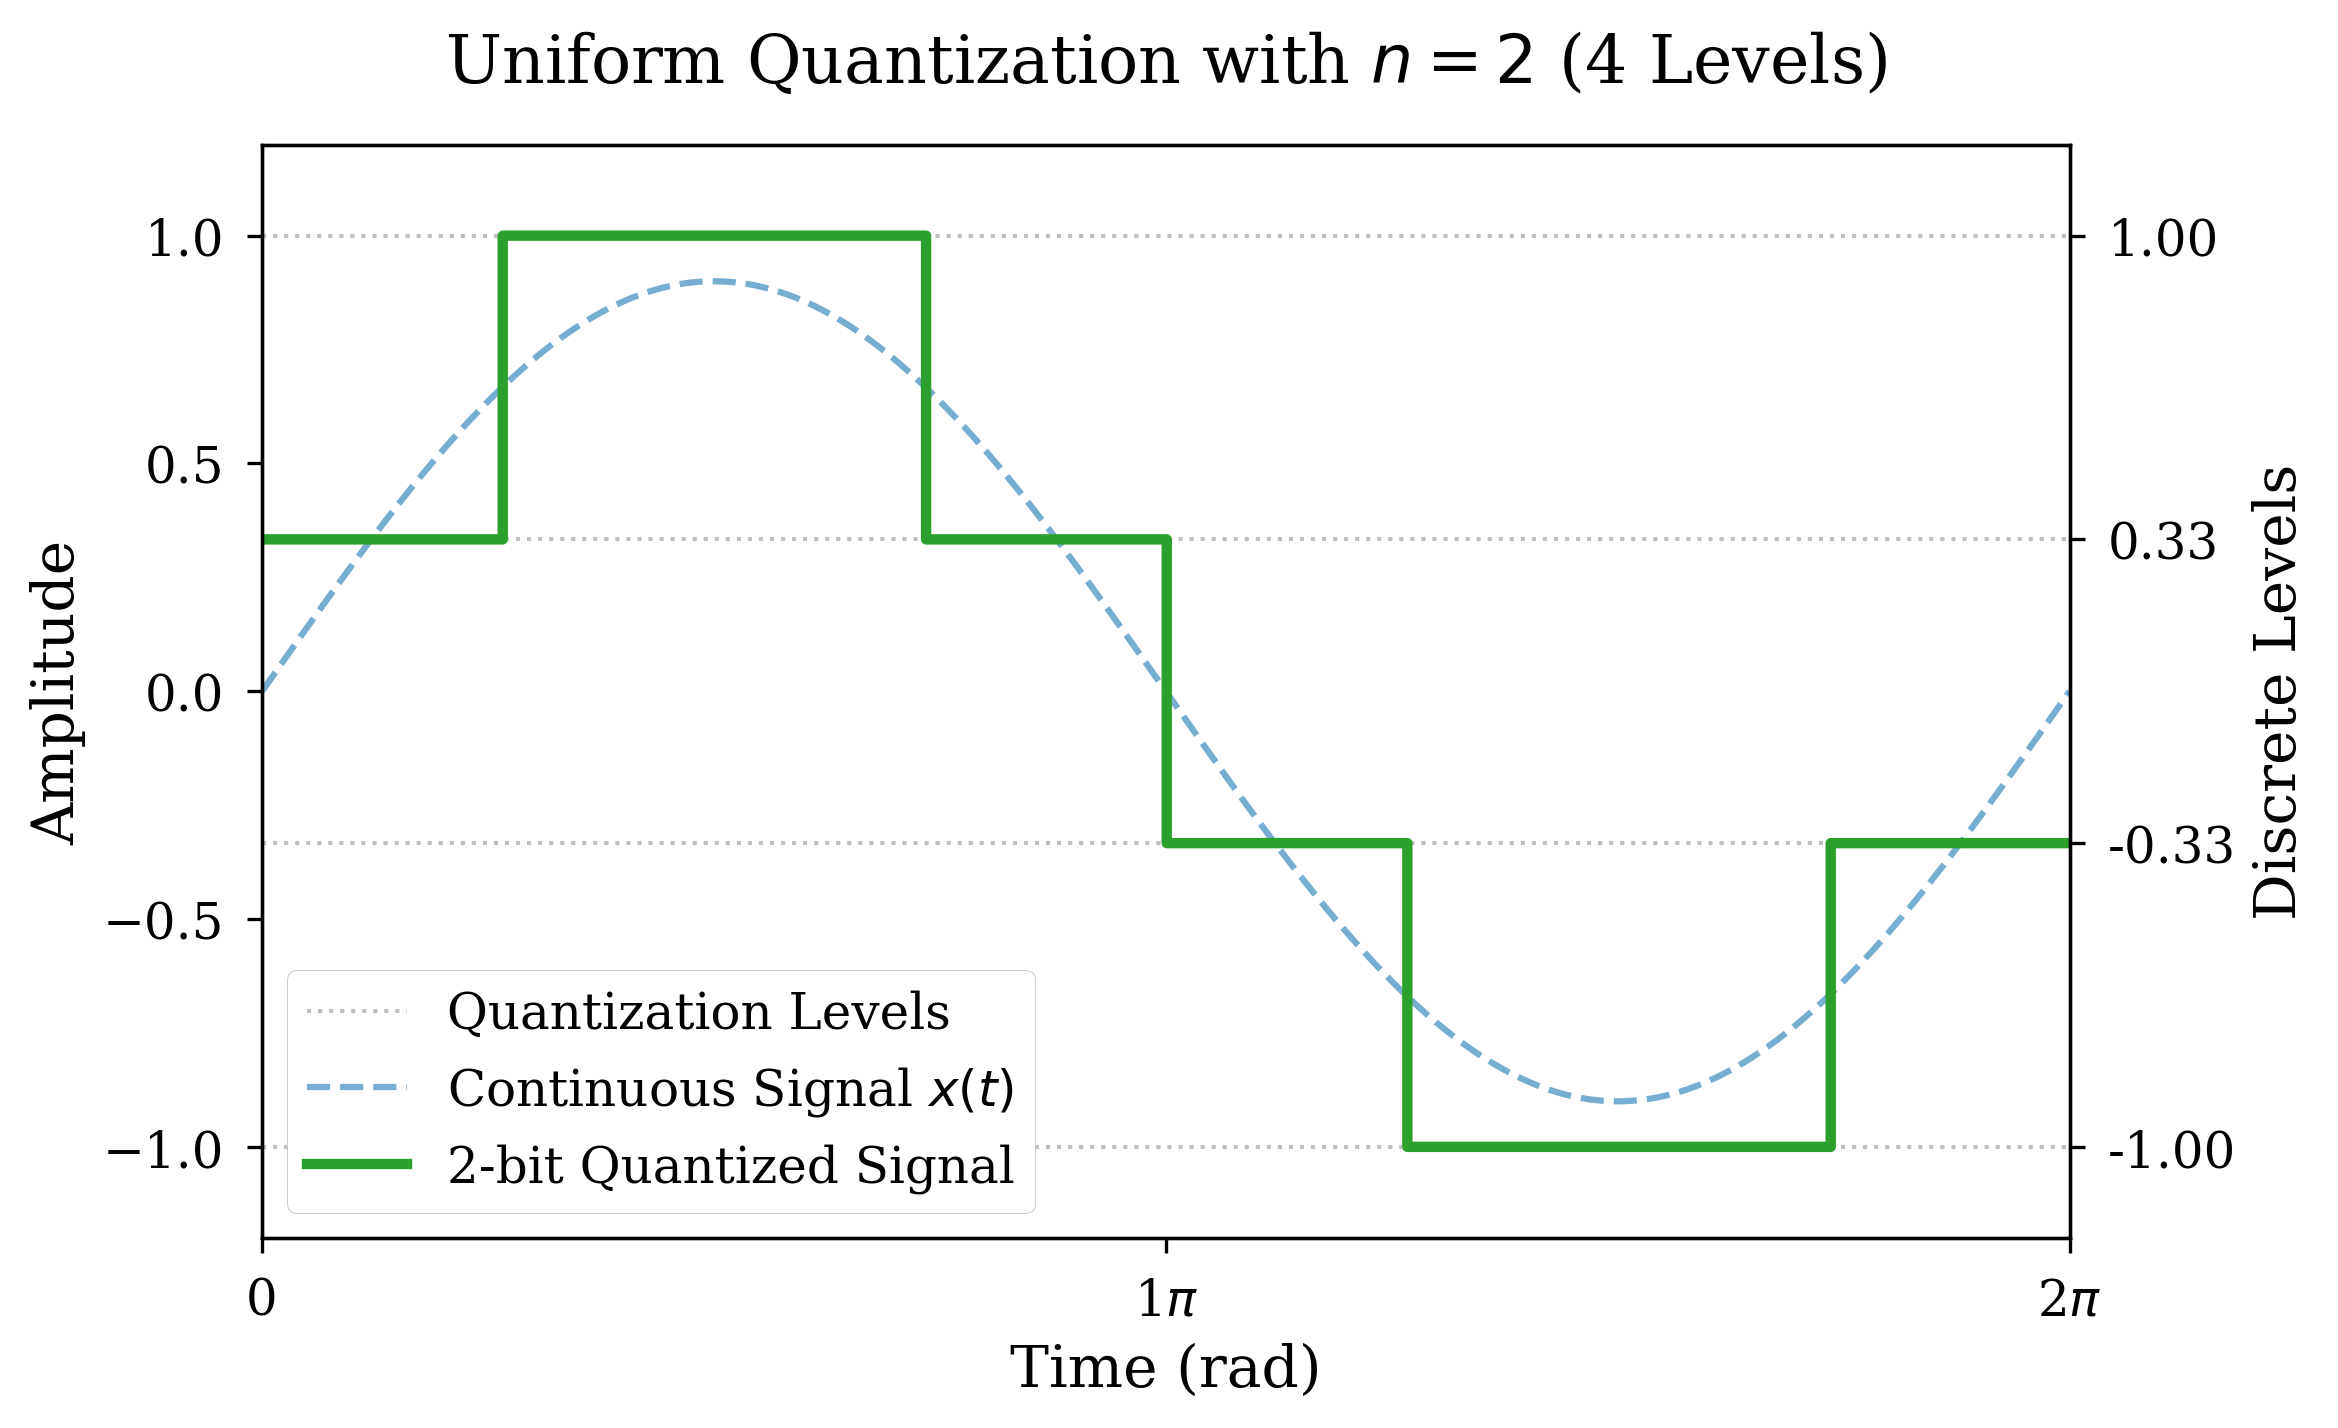
\includegraphics[width=0.75\linewidth]{figuras/2-fundamentos/quantization_n_2.png}
        \caption{Uniform quantization with $n=2$.}
        \label{fig:quant_n2}
    \end{minipage}
\end{figure}

\subsubsection*{Symmetric vs. Asymmetric Quantization}
These quantization strategies are classified as symmetric and asymmetric. In symmetric quantization, the zero-point is set to zero, and the scaling factor is applied evenly over the entire range of values, i.e., $\alpha = -\beta$. This approach is more simple and often sufficient for many applications, mainly when the distribution of values is approximately centered around zero. Consequently, symmetric quantization will be used throughout this work.

\begin{figure}[!ht]
\centering
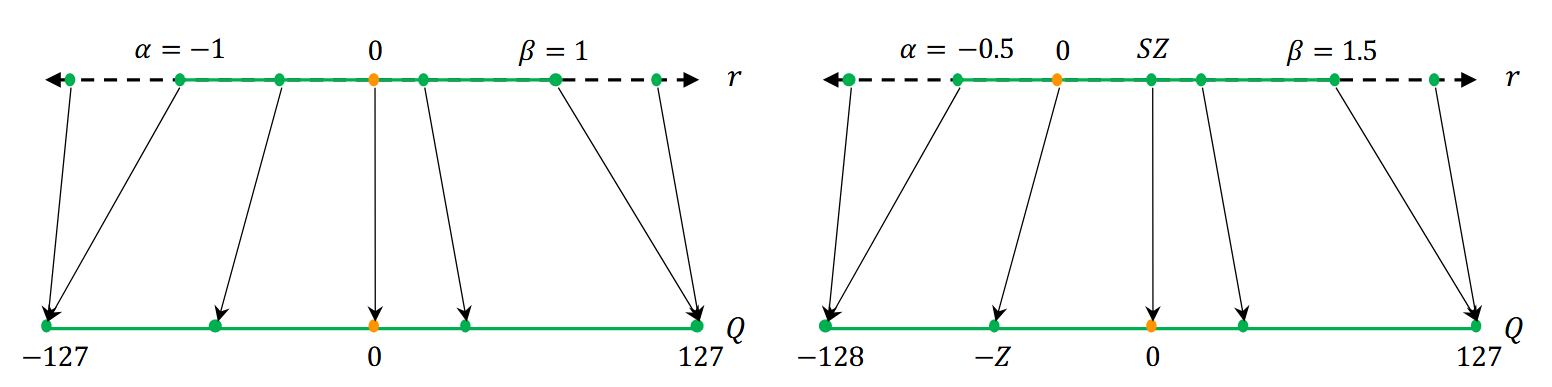
\includegraphics[width=0.8\textwidth]{figuras/2-fundamentos/quantization symetric.png}
\caption{Symmetric and asymmetric quantization.}
\label{fig:symmetric_quantization}
\end{figure}



Quantization strategies can be categorized as:
\begin{itemize}
    \item \textbf{Uniform vs. Non-uniform:} Uniform quantization uses equally spaced levels, while non-uniform uses samples from more densely populated regions.
    \item \textbf{Symmetric vs. Asymmetric:} Symmetric quantization has a zero point at zero, while asymmetric quantization allows for a non-zero zero point, which can better fit unbalanced distributions.
    %\item \textbf{Layer-wise vs. Channel-wise:} Layer-wise quantization applies a single quantization scheme to all parameters in a layer, while channel-wise quantization applies different schemes to each channel or filter, allowing for more flexibility and potentially better accuracy.
    \item \textbf{Fixed-point vs. Floating-point:} Fixed-point formats are more hardware-friendly and power-efficient, whereas low-bit floating-point formats (e.g., FP16, bfloat16) preserve a wider dynamic range.
\end{itemize}

The most crucial aspect of quantization in our scope is floating-point quantization, also called "fake quantization" \cite{gholami2021surveyquantizationmethodsefficient}, which simulates the effects of quantization during training, allowing the model to adapt and be represented in low-precision formats while maintaining the floating-point representation \cite{gholami2021surveyquantizationmethodsefficient}. Maintaining the floating-point representation \cite{gholami2021surveyquantizationmethodsefficient}. It therefore requires hardware to perform calculations in floating-point format, which is more flexible but less efficient than fixed-point arithmetic.

Fixed-point quantization represents numbers with a fixed number of bits for the integer and fractional parts, allowing for faster arithmetic operations and lower memory usage. This representation is most efficient when dealing with resource-constrained embedded devices\cite{sena2021verifying,gholami2021surveyquantizationmethodsefficient, huangEfficientVerificationQuantized2023}.

\subsection{ANN Quantization}

Strategies for quantizing ANNs are numerous, with many combinations of techniques \cite{jacob2018quantization, gholami2021surveyquantizationmethodsefficient}. The choice of strategy depends on the specific application, hardware constraints, and desired trade-offs between accuracy and efficiency. For this work, we will focus on quantizing the network’s parameters: weights, activation functions, and biases.

In general, we could use the equation \ref{eq:quantization} to quantize the weights, activations, and biases of a neural network. The quantization of the weights is performed layer by layer, where each layer $l$ has its own bit-width $n_l$:

\begin{equation}
W^{[l],q} = Q(n_l, W^{[l]}) \quad \text{for } l = 1, \dots, L,
\end{equation}
where $n_l$ is the bit-width for the $l$-th layer. The quantization of the biases follows a similar approach:
\begin{equation}
b^{[l],q} = Q(n_l, b^{[l]}) \quad \text{for } l = 1, \dots, L.
\end{equation}

However, there are considerations that must be taken into account when mapping each neural network element to the quantized representation. 

\subsubsection*{Weights}

Weights can be quantized using symmetric or asymmetric schemes \cite{gholami2021surveyquantizationmethodsefficient}. Symmetric quantization is widely adopted for weights because it simplifies the quantization function by setting the zero point ($Z$) to zero \cite{gholami2021surveyquantizationmethodsefficient}. This results in a simpler quantization function \ref{eq:quantization}, reducing computational cost during inference and making implementation more straightforward. In such cases, the clipping range is symmetric around zero, often chosen based on the maximum absolute weight. The ``full range'' approach (e.g., [-128, 127] for 8 bits) is generally more accurate than the "restricted range" (e.g., [-127, 127]) \cite{gholami2021surveyquantizationmethodsefficient}. On the other hand, asymmetric quantization uses a clipping range that is not necessarily symmetric and is preferred when weight distributions are unbalanced, as it can result in a tighter clipping range and better utilization of available bit width.

%The granularity of weight quantization is another critical factor. 
%\begin{itemize} 
%    \item Layerwise quantization applies a single clipping range to all weights within a layer. While simple to implement, it often results in sub-optimal accuracy if the range of individual convolutional filters varies widely. 
%    \item Groupwise quantization groups multiple channels within a layer to calculate the clipping range. This can be useful when parameter distributions vary significantly within a convolution but incurs an additional cost to account for different scaling factors. 
%    \item Channelwise quantization is the standard method for quantizing convolutional kernels. It assigns a dedicated scaling factor to each convolutional filter, ensuring better quantization resolution and often resulting in higher accuracy with negligible overhead. 
%    \item Sub-channelwise quantization offers the most granular control, but adds considerable overhead due to managing multiple scaling factors, making it less common. 
%\end{itemize}

Integer-only quantization, which is more desirable than simulated quantization. This is because all operations are performed using low-precision integer arithmetic \cite{gholami2021surveyquantizationmethodsefficient}, fully leveraging low-precision hardware logic that is faster, more power-efficient, and more area-efficient.

To mitigate post-quantization accuracy degradation, fine-tuning methods are employed. Quantization-Aware Training (QAT) involves retraining the model with quantized parameters to achieve lower loss and improved accuracy \cite{gholami2021surveyquantizationmethodsefficient}. QAT can also learn optimal quantization parameters, such as clipping ranges and weight scaling factors, during training. However, its main disadvantage is the high computational cost associated with extensive retraining. An alternative is Post-Training Quantization (PTQ), which quantizes and adjusts weights without retraining, offering very low, often negligible, overhead~\cite{gholami2021surveyquantizationmethodsefficient}. While faster, PTQ generally achieves lower accuracy than QAT~\cite{gholami2021surveyquantizationmethodsefficient}. For scenarios where no training/validation data is accessible, Zero-Shot Quantization (ZSQ) methods are used.

\begin{comment}
    
    Finally, to mitigate significant accuracy degradation in low-precision scenarios, mixed-precision quantization is utilized [62: \cite{gholami2021surveyquantizationmethodsefficient}; 65: \cite{gholami2021surveyquantizationmethodsefficient}]. This approach applies different bit precisions to different layers of the model [58: \cite{gholami2021surveyquantizationmethodsefficient}; 62: \cite{gholami2021surveyquantizationmethodsefficient}], with more sensitive layers kept at higher precision and less sensitive layers at lower precision [65: \cite{gholami2021surveyquantizationmethodsefficient}; 87: \cite{gholami2021surveyquantizationmethodsefficient}]. This aims to balance accuracy and efficiency across the model, minimizing accuracy degradation while still benefiting from reduced memory footprint and acceleration [65: \cite{gholami2021surveyquantizationmethodsefficient}]. Determining the optimal bit allocation per layer can involve complex search problems, such as reinforcement learning-based methods or Hessian-aware techniques [63: \cite{gholami2021surveyquantizationmethodsefficient}; 64: \cite{gholami2021surveyquantizationmethodsefficient}]. This approach has proven hardware-efficient, showing significant accelerations compared to uniform precision quantization [64: \cite{gholami2021surveyquantizationmethodsefficient}; 65: \cite{gholami2021surveyquantizationmethodsefficient}].
\end{comment}


\subsubsection*{Bias}



While the literature does not outline a single, standard quantization method for biases, there is a large discussion focused mainly on correction techniques \cite{gholami2021surveyquantizationmethodsefficient}. 

A known consequence of certain approaches, such as PTQ, is a shift in the means of the weight and activation values, which negatively impacts model accuracy. The solution lies in applying a bias correction method that seeks to readjust these deviations \cite{gholami2021surveyquantizationmethodsefficient}.

The choice between symmetric and asymmetric quantization directly influences this dynamic. In asymmetric quantization, where the clipping range is not necessarily centered at the origin, cross-terms emerge. As these terms are static, they can be absorbed by the layer's bias, thereby enabling practical hardware optimization. In contrast, symmetric quantization is inherently free of this issue, as its zero-centered range does not generate such terms.

Beyond these considerations, other techniques focus on making the neural network more amenable to quantization. Range Equalization, for example, normalizes the weight value ranges across layers, implicitly standardizing activations and lowering total error. The success of this technique is amplified in Zero-Shot Quantization scenarios, without the presence of calibration data makes bias error correction a fundamental step. Indeed, the most reliable approaches for quantization without training data often combine weight equalization and bias correction, therewith safeguarding the robustness of the quantized model.

\subsubsection*{Activations}

Quantizing activations depends on the activation function used in the ANN. For example, ReLU activations are typically quantized using symmetric quantization. Other activation functions may require asymmetric quantization. The process of quantizing activations is performed layer by layer. Each layer $l$ has its own bit-width $n_l$: 

\begin{equation}
A^{[l],q} = Q(n_l, A^{[l]}) \quad \text{for } l = 1, \dots, L,
\end{equation}

\begin{comment}
Quantizing each ANN parameter results in a loss of precision and accuracy in the quantized model due to numerical precision, known as the implementation gap between the idealized real-valued model and its finite-precision realization \cite{Cai2020Certified,cordeiro2025neuralnetworkverificationprogramming}. As discussed earlier, there are many variations in quantization. Symmetric quantization applies the same scale to the positive and negative values, while asymmetric quantization uses different scales or offsets. Uniform quantization assigns equal intervals between quantized values, whereas non-uniform quantization uses variable intervals \cite{gholami2021surveyquantizationmethodsefficient,gholami2021surveyquantizationmethodsefficient}. The number of bits used to quantize elements, as well as other techniques, also varies\cite{huangEfficientVerificationQuantized2023}. Each technique brings about a disturbance to the overall model. Considering this, safety properties were created for verification and to guide the selection of the best quantization approach for specific models.
    
\section{Vulnerabilities Introduced by Quantization}

Neural Networks have started to be used to replace work classifications that used to be done by human professionals, e.g., partten recognition professions like doctors. A computer, unlike a human, can deal with huge amounts of images and classify them as correctly as it should. However, due to new techniques of adversarial attack, the use of machine learning has become more 


Even small errors may lead to misclassification of the Neural Network due to the "error amplification effect," in which small residual adversarial noise is progressively amplified through the network's layers \cite{liaoDefenseAdversarialAttacks2018}.  

Quantization amplifies the pertubation, i.e., it makes the model more sensive to input pertubation \cite{zhangQEBVerifQuantizationError2023}, thus making the new model to misclassify more than the baseline one. It inherenly brings the model more successiable to adversarial attacks.

As explained by Sena et al. in \cite{sena2021verifying} because of less bit-width, any small pertubation may make significative changes on the hidden layers and then make the model to wronglly classify.

The quantization impacts on the decision borders \cite{gorslineAdversarialRobustnessQuantized2021}. During weight reduction, the netwroks loses the capability to define smooth borders and thus to have a precise inference between classes. This influences direcetly on gradient attacks, beacuse the attacker aims to hit the region where the missclassification happens \cite{gorslineAdversarialRobustnessQuantized2021}.

A concept defined by Giacobbe et al. in \cite{giacobbe2020how} proves that robustness is not non-monotonic bitwise, i.e., a 32 bit may become vulnerable if quantized to a 8 bit precision, but other model might as well become vulnerable if the precision is increased, e.g., from 6 to 8 for example. This phenomenon justifies the need to exist a bit-precision verification because anything can happen to a model by swapping the bit precision.

As discussed previously, Quantization introduces statistical errors into the Quantized model. These errors may affect the model's ability to classify and operate properly on input data. Thus, there is a need to assess safety features.
    My work relies on
ANNs and QNNs are like black boxes: in practice, we only control the input and observe the output, while the internal reasoning is not explicitly accessible. As a result, most safety and security properties naturally express as constraints on their input-output relations. Let $f$ be the network function mapping an input $x \in \mathcal{I}$ to an output space $\mathcal{O}$. Then, a generic safety requirement can be stated as: for every input $x \in \mathcal{I}$, the produced output must lie in a desired set $\mathcal{G}$, i.e., it must satisfy the property $P$:
\[
\forall x \in \mathcal{I} \;\Rightarrow\; f(x) \in \mathcal{G}.
\]

One important safety-related property is adversarial robustness. This property is usually regarded as the requirement that small perturbations in the input should not change the model decision. The predicted label must stay the same even if the input is slightly modified \cite{huangSurveySafetyTrustworthiness2020, linIntegerarithmeticonlyCertifiedRobustness2021}. Consider an input domain $\mathcal{D}$ and a neighborhood around a specific input $x \in \mathcal{D}$, defined by a metric $d_{\text{in}}$ and referred to as $\mathcal{I}(x,d_{\text{in}})$. If $y$ represents the correct label for $x$, robustness can be formalized as
\[
\forall  x' \in \mathcal{I}(x,d_{\text{in}}) \;\Rightarrow\; f(x') = y,
\] 

Here, $\mathcal{I}(x,d_{\text{in}})$ is typically constrained by a radius $\epsilon$. This means the distance between two values must be less than or equal to $\epsilon$, for example, $d_{\text{in}}(x,x') \le \epsilon$ \cite{huangSurveySafetyTrustworthiness2020}. This research uses an $L_\infty$ ball, which restricts the maximum deviation for each feature:
\[
\mathcal{I}(x,\epsilon) = \left\{ x' \in \mathbb{R}^n \;\middle|\; \|x - x'\|_\infty \le \epsilon \right\}.
\]
As defined in the survey \cite{huangSurveySafetyTrustworthiness2020} the adversarial attack can be defined as in Definition \ref{definition:adversarial_atttack}.
\begin{definition}[Adversarial Example]\label{definition:adversarial_atttack}
Given a ANN $f : \mathcal{I} \to \mathcal{O}$, a human decision oracle $\mathcal{H} : \mathcal I \to \mathcal{O}$, and a legitimate input $x \in \mathcal{I}$ with $\arg \max_j f_j(x) = \arg \max_j \mathcal{H}_j(x)$, an adversarial example to a ANN is defined as:
\begin{equation}
\begin{aligned}
\exists \hat{x} : \quad & \arg \max_j \mathcal{H}_j(\hat{x}) = \arg \max_j \mathcal{H}_j(x) \\
& \wedge ||x - \hat{x}||_p \leq d \\
& \wedge \arg \max_j f_j(\hat{x}) \neq \arg \max_j f_j(x)
\end{aligned}
\end{equation}
where $p \in \mathbb{N}, p \geq 1, d \in \mathbb{R}$, and $d > 0$.
\end{definition}

The cause of vulnerability to \textit{adversarial examples} is likely due to to extreme nonlinearity of Neural Network Models \cite{goodfellowExplainingHarnessingAdversarial2015}


%% New text
\subsection{Adversarial Attack Verification Using SMT}

In the context of NN, equivalence refers to the property that two neural networks can produce the same outputs given the same set of inputs. This is particularly important when considering the quantization process, which aims to reduce the network's size to fit the NN into a resource-constrained environment without significantly degrading its performance.

We define neural network equivalence in terms of their outputs over a given input space. Specifically, we consider two neural networks, $f$ and $t$, where $f$ is the original floating-point neural network and $t$ is the quantized neural network. The equivalence condition can be expressed as follows:
\begin{equation}
f(x) \sim t(x), \quad \forall x \in I,
\end{equation}
where $I$ is the input space and $O$ is the output space. This means that for every input $x$ in the input space, the output of the original neural network $f$ and the output of the quantized neural network $t$ must produce the same class label or output value.
\end{comment}

%
\section{Safety and Robustness in Quantized Neural Networks}

Neural Networks have begun to replace work previously performed by human professionals. For example, in pattern recognition, computers perform tasks similar to those of doctors. Unlike humans, a computer can process large numbers of images and classify them with high accuracy. However, new adversarial attack techniques have made the use of machine learning more challenging. Techniques such as Fast Gradient Sign Method (FGSM) \& R+FGSM \cite{goodfellowExplainingHarnessingAdversarial2015}, Random Perturbation, and Basic Interactive Method \cite{kurakin2017adversarialmachinelearningscale} allow an attacker to subtly alter the input data. These small perturbations, although imperceptible to humans, are specifically designed to cause the model to misclassify the input as defined in Definition \ref{definition:adversarial_attack} \cite{goodfellowExplainingHarnessingAdversarial2015}.
\newpage
\begin{figure}
    \centering
    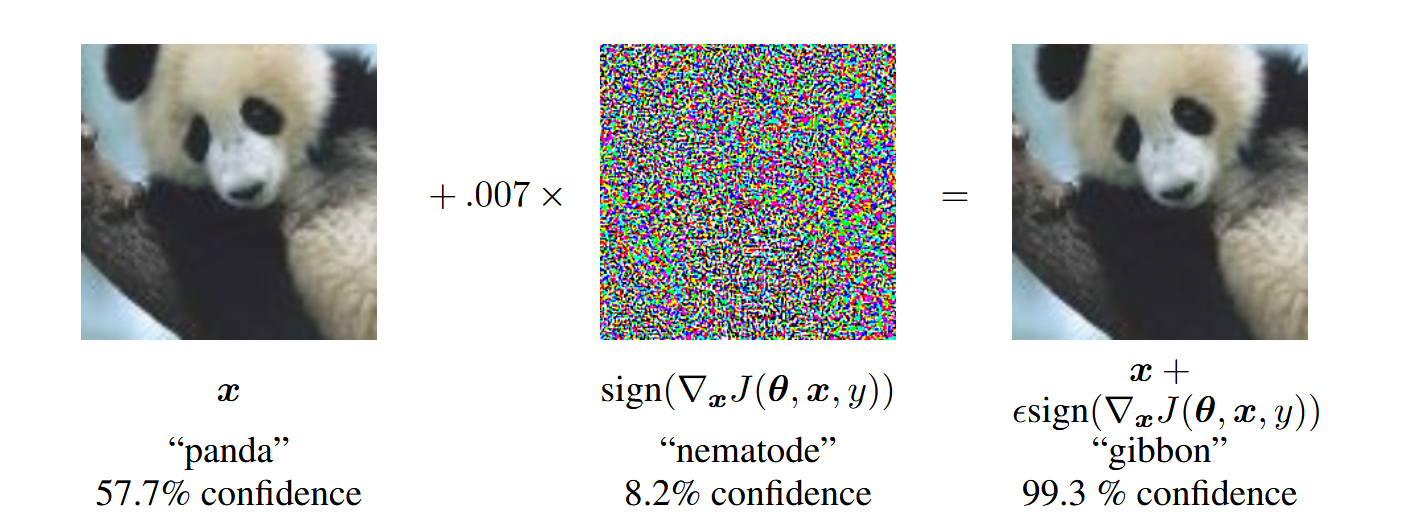
\includegraphics[width=1\textwidth]{figuras/2-fundamentos/safety/adversarial_attack_panda_example.png}
    \caption{Adversarial Attack Extracted from \cite{goodfellowExplainingHarnessingAdversarial2015}}
    \label{fig:panda_example_safety}
    \end{figure}
    
ANNs and QNNs are like black boxes: in practice, we only control the input and observe the output, while the internal reasoning is not explicitly accessible. As a result, most safety and security properties naturally express as constraints on their input-output relations. To formalize this, let $f$ be the network function mapping an input $x \in \mathcal{I}$ to an output space $\mathcal{O}$. Then, a generic safety requirement can be stated as: for every input $x \in \mathcal{I}$, the produced output must lie in a desired set $\mathcal{G}$, i.e., it must satisfy the property $P$:
\[
\forall x \in \mathcal{I} \;\Rightarrow\; f(x) \in \mathcal{G}.
\]

Building on this formal framework, one important safety-related property is adversarial robustness. This property is usually regarded as the requirement that small perturbations in the input should not change the model decision. The predicted label must stay the same even if the input is slightly modified \cite{huangSurveySafetyTrustworthiness2020, linIntegerarithmeticonlyCertifiedRobustness2021}. Consider an input domain $\mathcal{D}$ and a neighborhood around a specific input $x \in \mathcal{D}$, defined by a metric $d_{\text{in}}$ and referred to as $\mathcal{I}(x,d_{\text{in}})$. If $y$ represents the correct label for $x$, robustness can be formalized as:
\[
\forall  x' \in \mathcal{I}(x,d_{\text{in}}) \;\Rightarrow\; f(x') = y.
\] 

Here, $\mathcal{I}(x,d_{\text{in}})$ is typically constrained by a radius $\epsilon$. This means the distance between two values must be less than or equal to $\epsilon$, for example, $d_{\text{in}}(x,x') \le \epsilon$ \cite{huangSurveySafetyTrustworthiness2020}. This research uses an $L_\infty$ ball, which restricts the maximum deviation for each feature:
\[
\mathcal{I}(x,\epsilon) = \left\{ x' \in \mathbb{R}^n \;\middle|\; \|x - x'\|_\infty \le \epsilon \right\}.
\]

As defined in the survey \cite{huangSurveySafetyTrustworthiness2020}, the adversarial attack can be defined as in Definition \ref{definition:adversarial_attack}.

\begin{definition}[Adversarial Example]\label{definition:adversarial_attack}
Given an ANN $f : \mathcal{I} \to \mathcal{O}$, a human decision oracle $\mathcal{H} : \mathcal I \to \mathcal{O}$, and a legitimate input $x \in \mathcal{I}$ with $\arg \max_j f_j(x) = \arg \max_j \mathcal{H}_j(x)$, an adversarial example to an ANN is defined as:
\begin{equation}
\begin{aligned}
\exists \hat{x} : \quad & \arg \max_j \mathcal{H}_j(\hat{x}) = \arg \max_j \mathcal{H}_j(x) \\
& \wedge ||x - \hat{x}||_p \leq d \\
& \wedge \arg \max_j f_j(\hat{x}) \neq \arg \max_j f_j(x)
\end{aligned}
\end{equation}
where $p \in \mathbb{N}, p \geq 1, d \in \mathbb{R}$, and $d > 0$.
\end{definition}

The cause of vulnerability to \textit{adversarial examples} is likely due to the extreme nonlinearity of Neural Network Models \cite{goodfellowExplainingHarnessingAdversarial2015}. Even small errors may lead to misclassification of the Neural Network due to the "error amplification effect," in which small residual adversarial noise is progressively amplified through the network's layers \cite{liaoDefenseAdversarialAttacks2018}.  

\subsection*{Quantization and Robustness}
As discussed previously, Quantization introduces statistical errors into the Quantized model. These errors may affect the model's ability to classify and operate properly on input data. Thus, there is a need to assess safety features. Quantization amplifies the perturbation, i.e., it makes the model more sensitive to input perturbations \cite{zhangQEBVerifQuantizationError2023}, thereby leading the new model to misclassify more frequently than the baseline one. It inherently makes the model more susceptible to adversarial attacks. As explained by Sena et al. in \cite{sena2021verifying}, due to lower bit-width, even small perturbations can significantly alter hidden-layer activations, leading the model to misclassify.

Additionally, quantization affects decision boundaries \cite{gorslineAdversarialRobustnessQuantized2021}. During weight reduction, the network loses the ability to define smooth boundaries and thus to perform precise class inference. This directly influences gradient-based attacks, because the attacker aims to hit the region where misclassification occurs \cite{gorslineAdversarialRobustnessQuantized2021}.

In the work of \cite{goodfellowExplainingHarnessingAdversarial2015}, it's shown that the accuracy drop happens later than the adversarial vulnerability: It states that with quantization, the accuracy of the model in the work does not drop until a 4-bit bit-width is chosen, though the drop happens with 5 bit-width when attacked by the adversarial attack, dropping by 25\% the accuracy of the model.

Further supporting the need for careful analysis, a concept defined by Giacobbe et al. in \cite{giacobbe2020how} proves that robustness is not non-monotonic bitwise, i.e., a 32-bit model may become vulnerable if quantized to 8-bit precision, but another model might as well become vulnerable if the precision is increased, e.g., from 6 to 8. This phenomenon underscores the need for bit-precision verification, as anything can happen to a model when bit precision is swapped.


\section{Safety and Robustness in Quantized Neural Networks}

Neural Networks have begun to replace work previously performed by human professionals. For example, in pattern recognition, computers perform tasks similar to those of doctors. Unlike humans, a computer can process large numbers of images and classify them with high accuracy. However, new adversarial attack techniques have made the use of machine learning more challenging. Techniques such as Fast Gradient Sign Method (FGSM) \& R+FGSM \cite{goodfellowExplainingHarnessingAdversarial2015}, Random Perturbation, and Basic Interactive Method \cite{kurakin2017adversarialmachinelearningscale} allow the attacker to subtly alter the input data. These small perturbations, although imperceptible to humans, are specifically designed to cause the model to misclassify the input as defined in Definition \ref{definition:adversarial_attack} \cite{goodfellowExplainingHarnessingAdversarial2015} and seen in Figure \ref{fig:panda_example_safety}.

\newpage
\begin{figure}[!ht]
    \centering
    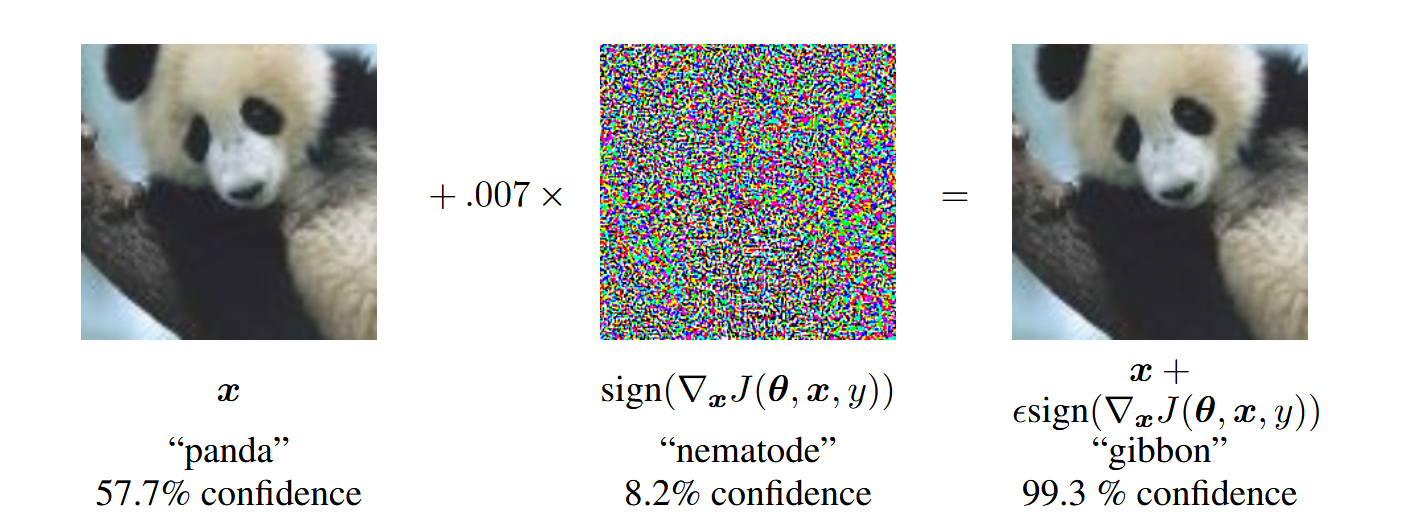
\includegraphics[width=0.8\textwidth]{figuras/2-fundamentos/safety/adversarial_attack_panda_example.png}
    \caption{Example of an adversarial Attack when a noise induces the decision maker to misclassify \cite{goodfellowExplainingHarnessingAdversarial2015}}
    \label{fig:panda_example_safety}
\end{figure}

In simpler words:
\begin{equation}
    original + perturbation = attack
\end{equation}
    
ANNs and QNNs are like black boxes: in practice, we only control the input and observe the output, while the internal reasoning is not explicitly accessible. As a result, most safety and security properties naturally express as constraints on their input-output relations. To formalize this, let $f$ be the network function mapping an input $x \in \mathcal{I}$ to an output space $\mathcal{O}$. Then, a generic safety requirement can be stated as: for every input $x \in \mathcal{I}$, the produced output must lie in a desired set $\mathcal{G}$, i.e., it must satisfy the property $\Phi$:

\begin{equation}\label{eq:security_gen_prop}
%\forall x \in \mathcal{I} \;\Rightarrow\; f(x) \in \mathcal{G}.    
 \forall \mathbf{x} \in \mathcal{I}, \quad f(\mathbf{x}) \in \mathcal{G}
 \end{equation}


It is very important to make a clear ditiguish between global and local robustness. The Equation \ref{eq:security_gen_prop} described the former by implying verification of the whole input space. However, it would lead to state explosions, as there are a infinite number of valid inputs \cite{huangSafetyVerificationDeep2017}. Consequently, formal verification often retricts is scope to a small set of training data to prove local robustness around that points. 

Building on this formal framework, one important safety-related property is local adversarial robustness. This property is usually regarded as the requirement that small perturbations in the input should not change the model decision. The predicted label must stay the same even if the input is slightly modified \cite{huangSurveySafetyTrustworthiness2020, linIntegerarithmeticonlyCertifiedRobustness2021}. Consider an input domain $\mathcal{I}$ and a neighborhood around a specific input $x \in \mathcal{I}$, defined by a metric $d_{\text{in}}$ and referred to as $\mathcal{I}(x,d_{\text{in}})$. If $y$ represents the correct label for $x$, robustness can be formalized as:
\begin{equation}\label{eq:local_robustness}
 \forall \, \mathbf{x}' \in \mathcal{B}_\infty(\mathbf{x}, \epsilon), \quad \arg\max f(\mathbf{x}') = \arg\max f(\mathbf{x}) 
\end{equation}


Here, $\mathcal{B}(x,\epsilon)$ is typically constrained by a radius $\epsilon$. This means the distance between two values must be less than or equal to $\epsilon$, for example, $d_{\text{in}}(x,x') \le \epsilon$ \cite{huangSurveySafetyTrustworthiness2020}. This research uses an $\ell_\infty$ ball, which restricts the maximum deviation for each feature:
\[
 \text{where } \mathcal{B}_{\infty}(\mathbf{x}, \epsilon) = \{\mathbf{x}' : \|\mathbf{x}' - \mathbf{x}\|_\infty \leq \epsilon\}
\] 

As defined in the survey \cite{huangSurveySafetyTrustworthiness2020}, the adversarial attack can be defined as in Definition \ref{definition:adversarial_attack}.

\begin{definition}[Adversarial Example]\label{definition:adversarial_attack}
Given an ANN $f : \mathcal{I} \to \mathcal{O}$, a human decision oracle $\mathcal{H} : \mathcal I \to \mathcal{O}$, and a legitimate input $x \in \mathcal{I}$ with $\arg \max_j f_j(x) = \arg \max_j \mathcal{H}_j(x)$, an adversarial example to an ANN is defined as:
\begin{equation}
\begin{aligned}
\exists \, \hat{x} : \quad & \arg \max_j \mathcal{H}_j(\hat{x}) = \arg \max_j \mathcal{H}_j(x) \\
& \wedge ||x - \hat{x}||_{\infty} \leq d_{in} \\
& \wedge \arg \max_j f_j(\hat{x}) \neq \arg \max_j f_j(x)
\end{aligned}
\end{equation}
\end{definition}

\textcolor{blue}{The equation above will be replaced by the below}


The cause of vulnerability to \textit{adversarial examples} is likely due to the extreme nonlinearity of Neural Network Models \cite{goodfellowExplainingHarnessingAdversarial2015}. Even small errors may lead to misclassification of the Neural Network due to the "error amplification effect," in which small residual adversarial noise is progressively amplified through the network's layers \cite{liaoDefenseAdversarialAttacks2018}.  

\subsection*{Quantization and Robustness Against Adversarial Attack}
As discussed previously, Quantization introduces statistical errors into the Quantized model. These errors may affect the model's ability to classify and operate properly on input data. Thus, there is a need to assess safety features. Quantization amplifies the perturbation, i.e., it makes the model more sensitive to input perturbations \cite{zhangQEBVerifQuantizationError2023}, thereby leading the new model to misclassify more frequently than the baseline one. It inherently makes the model more susceptible to adversarial attacks. As explained by Sena et al. in \cite{sena2021verifying}, due to lower bit-width, even small perturbations can significantly alter hidden-layer activations, leading the model to misclassify.

Additionally, quantization affects decision boundaries \cite{gorslineAdversarialRobustnessQuantized2021}. During weight reduction, the network loses the ability to define smooth boundaries and thus to perform precise class inference. This directly influences gradient-based attacks, because the attacker aims to hit the region where misclassification occurs \cite{gorslineAdversarialRobustnessQuantized2021}.

%In the work of Goodfellow et al. \cite{goodfellowExplainingHarnessingAdversarial2015}, it's shown that the accuracy drop happens later than the adversarial vulnerability: It states that with quantization, the accuracy of the model in the work does not drop until a 4-bit bit-width is chosen, though the drop happens with 5 bit-width when attacked by the adversarial attack, dropping by 25\% the accuracy of the model.
The experiments conducted by Goodfellow et al. \cite{goodfellowExplainingHarnessingAdversarial2015} show that, in Quantized models, the accuracy on the training dataset remains almost unchanged until 4-bit quantization is used. However, unlike the previous result, once an adversarial attack is induced, the accuracy drop occurs much earlier at 5 bit-width, dropping by 25\%. It shows that the model, once quantized, will not suffer from accuracy loss but will become much more vulnerable to adversarial attacks.

Further supporting the need for careful analysis, a concept defined by Giacobbe et al. in \cite{giacobbe2020how} proves that robustness is not nonmonotonic bitwise, i.e., the NN behavior after quantization is unpredictable, a 32-bit model may become vulnerable if quantized to 8-bit precision, whereas another model might as well become vulnerable if the precision is increased, e.g., from 6 to 8 bit-width. This phenomenon underscores the need for bit-precision verification, as anything can happen to a model when bit precision is swapped.

\section{Formal Verification of Quantized Neural Networks}
\begin{comment}
    
The story of Formal Verification started by Schuele and Schneider \cite{article_schule_schneider} which stabilied the based of Bound Model Checking to finite states. And though the focus wasn't to verify ANN, they introduced crucial ideas as reduct the problem of verification to a problem of logical satisfiability. These techniques is what would later allow to reduct the verification problem to an SMT problem years later.

Following this breakthrough,  Pulina et al. \cite{pulinaAbstractionRefinementApproachVerification2010} were the pioneer to use SMT verification in MLPs



To proactively prevent network vulnerabilities, a new verification area was established or revived. This development followed the findings of \cite{gorslineAdversarialRobustnessQuantized2021, kurakin2017adversarialmachinelearningscale}. These attacks intentionally mislead critical systems into incorrect classifications to achieve malicious goals. As a reprisal, several methods were developed to investigate the issue. In our line of work, we will focus on the works that use constraints to define security properties called deterministic guarantees \cite{gholami2021surveyquantizationmethodsefficient}.


\textit{Deterministic} guarantees are realized by transforming the verification problem into a set of constraints (e.g., asserts and assume statements) to be solved by a constraint solver, e.g, MILP solvers or SAT/SMT solvers. The name deterministic comes from the fact that these solvers return a deterministic answer to a query, i.e., either satisfiable or unsatisfiable \cite{gholami2021surveyquantizationmethodsefficient}.

The goal would be to use SMT solvers to verify properties like \ref{eq:security_gen_prop}.

SMT used in the literature extends to Z3, CV4, and Boolevector.

Recent works have shown that verifying Neural Networks with bit-precision is a PS-Hard task \cite{henzinger2021scalable}, thus harder than verifying floating-point Neural Networks.

Baranowski et al. developed a new background theory for fixed-point representation to be verified \cite{baranowski2020smt} that would be ideal to verify with bit-precision QNNs, as the 

SMT has been used to verify robustness from adversarial attacks 

Katz et al. introduced Reluplex to check local robustness on neural networks that use ReLu activation function, and it proves that small perturbations $\ell_\infty$ do not bring about misclassification \cite{katz2017reluplex}. Later Katz et al. and Wu et al. created a new framework called Marabou to verify adversarial robustness at large-scale neural networks. It expanded Reluplex to support any activation fuction \cite{katz2017reluplex, katz2019marabou, wuMarabou20Versatile2024}

Like our work, Huang et al. proposed verification of robustness layer-by-layer \cite{huangSafetyVerificationDeep2017}.

The first work to work with a robustness check of a Quantized Neural Network was Giacobbe, Henzinger, and Lechner at \cite{giacobbe2020how, henzinger2021scalable}. They introduced the use of bit vector theory to verify bit-precise and were the first to demonstrate that the quantization is not monotonic, thus the increase in bit precision can counter-intuitively increase the vulnerability of the model.

Amir et al. extended Marabou  to support $sign(x)$ activation function for the first time and also worked with binarized layers, which is a special case of quantization as it requires only one bit of precision.

among other works such such as \cite{song2021qnnverifier, sena2021verifying}

\subsection{SMT encoding}
In order to verify NN with bit-precision, the NN must be transformed to a code problem instead of a model problem, as it will be embarked into specific hardware, thus the first step is to transform the model into a C code \cite{cordeiro2025neuralnetworkverificationprogramming}. Once into C code, the next step is to transform the constraints into a satisfiability problem, i.e., encode the neural network layer ${f}_{n}$ into an SMT formula that will verify if by inputting a perturbation $\epsilon$ the known layer will be misclassified.
\end{comment}

%%%
The story of Formal Verification started by Schuele and Schneider \cite{article_schule_schneider}, which established the basis of Bounded Model Checking for finite states. Although their focus wasn't to verify {ANNs}, they introduced crucial ideas, such as reducing the verification problem to a problem of logical satisfiability. These techniques are what would later allow reducing the verification problem to an SMT problem years later. Following this breakthrough, Pulina et al. \cite{pulinaAbstractionRefinementApproachVerification2010} were the pioneers in using SMT verification for MLPs.

To proactively prevent network vulnerabilities, a new verification area was established or revived. This development followed the findings of \cite{gorslineAdversarialRobustnessQuantized2021, kurakin2017adversarialmachinelearningscale}, which showed that attacks can intentionally mislead critical systems into incorrect classifications to achieve malicious goals. In response, several methods were developed to investigate the issue. In our line of work, we will focus on works that use constraints to define security properties called deterministic guarantees \cite{gholami2021surveyquantizationmethodsefficient}.

{Deterministic} guarantees are realized by transforming the verification problem into a set of constraints (e.g., \texttt{assert} and \texttt{assume} statements) to be solved by a constraint solver, e.g., MILP solvers or SAT/SMT solvers. The name "deterministic" comes from the fact that these solvers return a deterministic answer to a query, i.e., either \textit{satisfiable} or \textit{unsatisfiable} \cite{gholami2021surveyquantizationmethodsefficient}. The goal is to use SMT solvers to verify properties like Equation \ref{eq:security_gen_prop}. SMT solvers used in the literature extend to Z3 , CVC4, and Boolector \cite{de2008z3, barrett2011cvc4, brummayer2009boolector} as solvable backend.

Recent works have shown that verifying Neural Networks with bit-precision is PSPACE-hard \cite{henzinger2021scalable}, making it harder than verifying floating-point Neural Networks. However, Baranowski et al. developed a new background theory for fixed-point representation \cite{baranowski2020smt} that is ideal for verifying bit-precision QNNs. This theory was integrated into off-the-shelf ESBMC, enabling QNN operations to be treated as verifiable C code \cite{song2021qnnverifier}. Through Operational Models, ESBMC faithfully captures the effects of rounding and overflow, enabling the search for adversarial counterexamples to account for the finite precision of the target hardware. Thus, the implementation in ESBMC resolves the semantic inconsistencies common to verifiers based on real representations, providing robustness guarantees that are solid for a deployment-constrained system.

SMT has been used extensively to verify robustness against adversarial attacks. Katz et al. introduced Reluplex to check local robustness on neural networks that use the ReLU activation function, proving that small perturbations $\ell_\infty$ do not bring about misclassification \cite{katz2017reluplex}. Later, Katz et al. and Wu et al. created a new framework called Marabou to verify adversarial robustness for large-scale neural networks, expanding Reluplex to support any activation function \cite{katz2017reluplex, katz2019marabou, wuMarabou20Versatile2024}. Like our work, Huang et al. proposed verification of robustness layer-by-layer \cite{huangSafetyVerificationDeep2017}.

The first work to address the robustness check of a Quantized Neural Network was by Giacobbe and Henzinger \cite{giacobbe2020how, henzinger2021scalable}. They introduced the use of bit-vector theory to verify bit-precision and were the first to demonstrate that quantization is nonmonotonic; thus, an increase in bit precision can counter-intuitively increase the vulnerability of the model. Amir et al. extended Marabou to support the $sign(x)$ activation function for the first time and also worked with binarized layers, which is a special case of quantization as it requires only one bit of precision. This field includes other works such as \cite{song2021qnnverifier, sena2021verifying}.

Instead of relying on heuristic adversarial attacks like FGSM to assess robustness, this work will use $\ell_\infty$-norm ball perturbation as it is more aligned with other formal methods in the literature \cite{cai2025certified, sena2021verifying}, as Gradient-based attacks (like PGD or JSMA) are incomplete, i.e., they can find vulnerabilities, but cannot prove their absence \cite{huangSafetyVerificationDeep2017}. It will allow our framework to verify whether, under a uniform-interval perturbation $\epsilon$, the network is safe and sound; therefore, allowing us to verify the local robustness property \ref{eq:local_robustness}. The affirmation can be visually checked in the Figure \ref{fig:uniform_norm_verification}.

\begin{figure}[!ht]
    \centering
    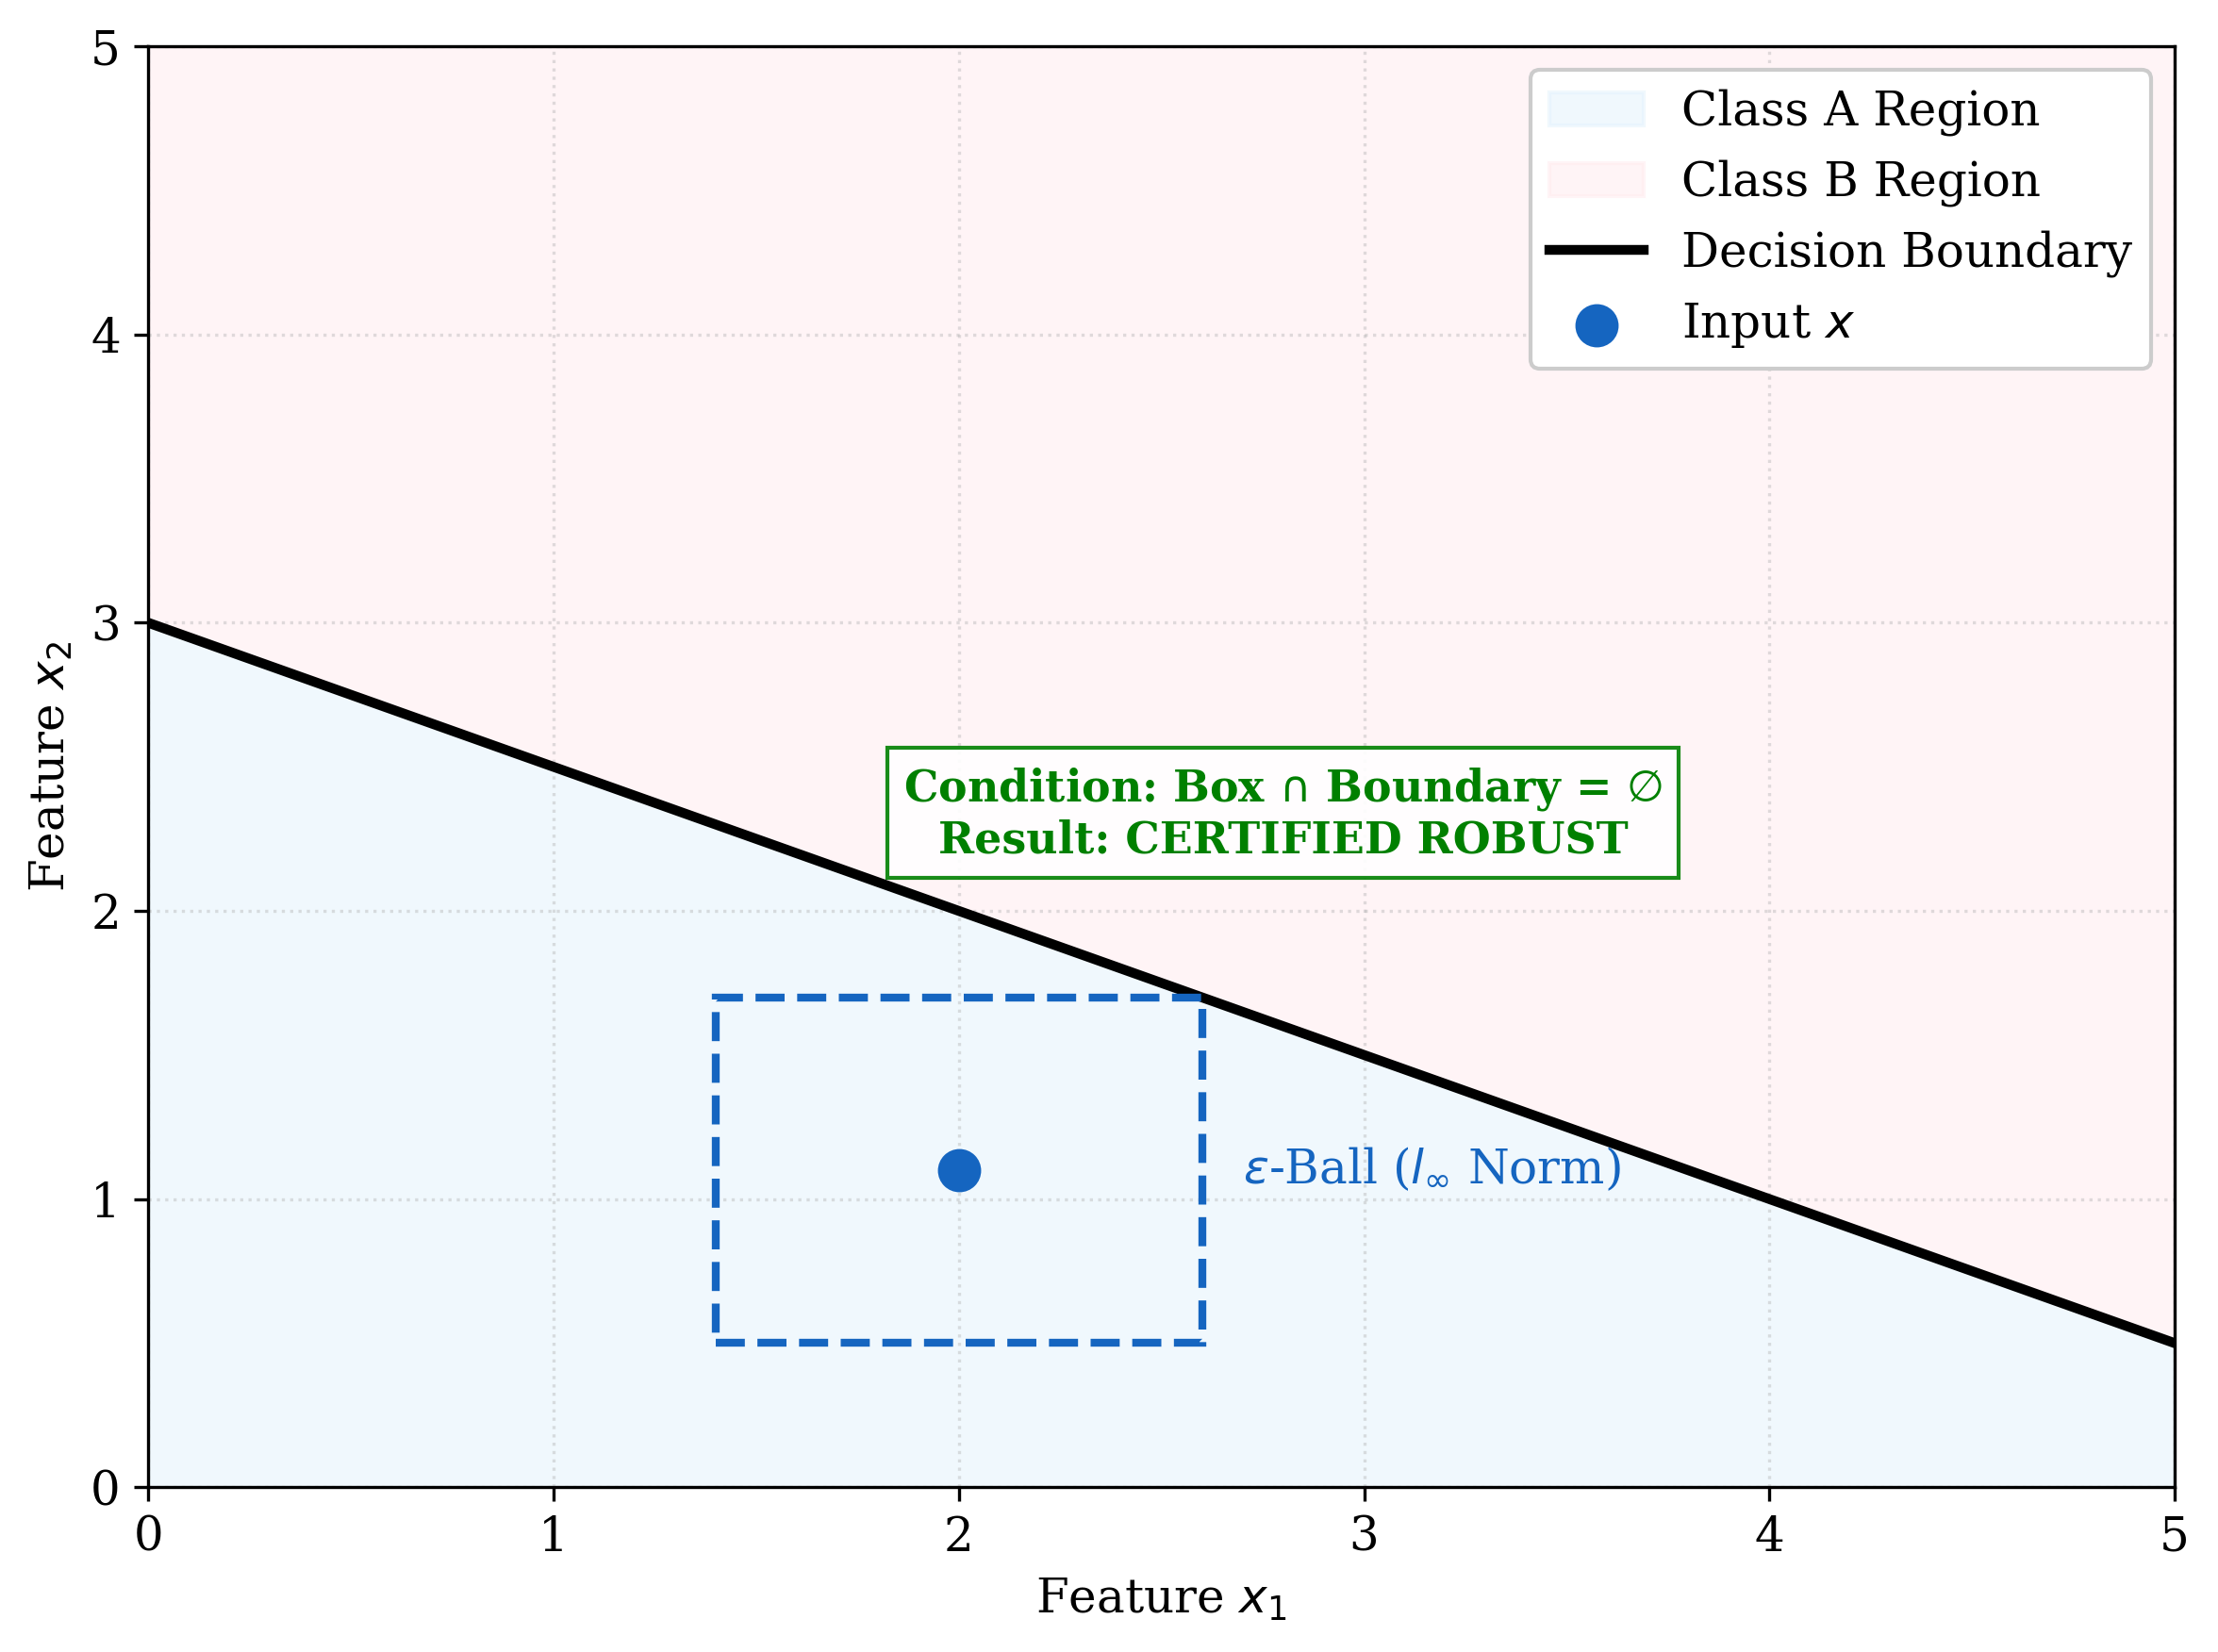
\includegraphics[width=0.8\textwidth]{figuras/2-fundamentos/safety/fig_why_uniform_linf.png}
    \caption{Example of $\ell_\infty$-norm ball}
    \label{fig:uniform_norm_verification}
    \end{figure}


\subsection{SMT Encoding}
In order to verify {QNNs} with bit-precision, the network must be transformed into a code problem rather than a model problem. As it will be embedded onto specific hardware, the first step is to transform the model into C code \cite{cordeiro2025neuralnetworkverificationprogramming}. Once in C code, the next step is to transform the constraints into a satisfiability problem, i.e., encode the neural network layer $f^{[l]}$ into an SMT formula that will verify if, by inputting a perturbation $\epsilon$, the known layer will be misclassified.

\begin{equation}
    \textbf{x}' = \textbf{x}+\epsilon,
\end{equation}
\begin{equation} \label{eq:safety_prop}
    \exists \, \textbf{x}' \in \mathcal{I} \rightarrow f'(\textbf{x}')\notin \mathcal{O}
\end{equation}

SMT solvers work by defining equations and constraints; we must write the safety property as a negation, i.e., a counterexample to be found. To use the Equation \ref{eq:safety_prop} with SMT solvers, it must be written as constraints:

\begin{align*}
\Phi_{\text{robust}}(\mathbf{x}, \epsilon) = & \exists \, \mathbf{x}' \in \mathcal{I} : \\
& \bigwedge_{i=1}^n (x_i - \epsilon \leq x'_i \leq x_i + \epsilon) \ \land \\
& \lnot (\arg\max \hat{f}(\mathbf{x}') \equiv \arg\max \hat{f}(\mathbf{x}))
\end{align*}
    
\begin{comment}
\subsubsection*{CEG4N}


\textbf{Neural Networks:} $\Gamma$ and $F$ \\
\textbf{Input Space:} $I \in \mathbb{R}^n$ \\
\textbf{Output Space:} $O \in \mathbb{R}^n$ \\

\textbf{Objective:} Prove that the mathematical functions of $\Gamma$ and $F$, $f:I \rightarrow O$ and $t:I\rightarrow O$, are equivalent.

\textbf{Equivalence:} Both NNs produce the same outputs for the same inputs.

\textbf{Definition 1 (Top-1-Equivalence):} Two NNs $f$ and $t$ are Top-1-equivalent if:
$$ \arg\max f(x) = \arg\max t(x), \forall x \in I $$

\textbf{Assumption 1:} For NN $F$ without quantization:
$$ \arg\max f(x) = y, \text{ for } x \in H $$

\textbf{Assumption 2:} For NN $F$ with quantization:
$$ \exists N \text{ such that } \arg\max f(x) = \arg\max f^q(x) = y, \forall x \in H $$



\textbf{Objective:} Maximize quantization while maintaining QNN equivalence to the floating point NN.

\textbf{Definition 2 (Robust Quantization):}
Let \( f \) be the reference NN and \( H \subset \mathbb{R}^n \) be a set of instances. Robust quantization is defined as:
\[ \text{Quantization of } f \text{ resulting in } f^q \text{ such that } \arg\max f(x) \Leftrightarrow \arg\max f^q(x), \forall x \in H \]

\textbf{Quantization Assumption:}
There exists a set \( N = \{n_1, n_2, \ldots, n_L\} \), where \( n_l \in N \) represents the number of bits for quantizing the \( l \)-th layer in \( f \).

\textbf{Robust Quantization Problem:}
Obtain a sequence of \( N \) where each \( n \in N \) is minimized, ensuring the equivalence between \( f \) and \( f^q \) is satisfied.


We consider the robust quantization of a neural network (NN) as an iterative minimization problem. Each iteration consists of two complementary sub-problems:

\begin{enumerate}
  \item Minimize the quantization bit widths by finding a candidate set \( N \).
  \item Verify the equivalence property, i.e., check if an NN quantized with the bit widths in \( N \) is equivalent to the original NN.
\end{enumerate}

\textbf{If the latter fails, we iteratively return to the minimization sub-problem with additional information.}

\begin{equation}
    N^o = \arg\min_{n_1,...,n_L} \sum_{l \in N_l <= L} n_l 
\end{equation}
    
$$
\begin{aligned}
& \arg\max f(x) = \arg\max f^q(x), & \forall x \in H^o_{CE} \\
& n_l \geq \underline{N} \vee n_l  \in N^o \\
& n_l  \leq \overline{N}  \vee n_l  \in N^o 
\end{aligned}
$$
    

Consider \( \overline{N} \) to be the upper limit and \( \underline{N} \) the lower one.
\begin{itemize}
  \item \( \overline{N} \) ensures two things:
  \begin{enumerate}
    \item It gives an upper bound to the quantization bit width.
    \item It provides a termination criterion. If a candidate \( N^o \) is found such that \( n_l = \overline{N} \) for every \( n_l \in N^o \), the optimization stops as it reaches Assumption 2.
  \end{enumerate}
  \item Assumption 2 ensures the termination of CEG4N, built on the premise that there exists a set of \( N \) where quantization introduces minimal error to the NN.
  \item If CEG4N proposes a quantization solution equal to \( \overline{N} \), this solution is verified, and if verification returns a counter-example, CEG4N finishes with failure.
  \item Note that \( H^o_{CE} \) is an iterative parameter, updated at each iteration based on the verification sub-problem.
\end{itemize}

In the Verification sub-problem $o$, we check whether the $N^o$ generated by the optimization sub-problem $o$ satisfies the following equivalence property:

\[\Psi(f,f^q, x,y)=\Psi_x(x)\rightarrow \Psi_y(y)\]

if  $\Psi_x(x)\rightarrow \Psi_y(y)$ holds for the candidate $N^o$, the optimization halts and $N^o$ is declared as solution; otherwise, a new counter-example $H_{CE}$ is generated. Iteration o+1 starts where iteration o stopped. That is, the optimization sub-problem o + 1 receives as parameter a set of $H^{+1}_{CE}$ such that $H^{o+1}_{CE}=H^o_{CE}\cup x_{CE}$.

    
    \subsection{Problem Encoding}
    
    \subsection{Neural Network Equivalence Problem}
    
    
    \subsection{Network Repair}
    
    Like said before, QNN are widely employed in human-activity. However, the quantization process can lead to a significant loss of accuracy. To address this issue, researchers have explored various techniques to repair quantized neural networks (QNNs).
    
    Repair NN have two main objectives: fix defects found in Neural Networks. It can be classified into three categories: retraining/fine-tuning, direct weight modification, and architecture extension \cite{song2023qnnrepair}.
    
    The equivalence problem is a fundamental challenge in the field of neural Network Repair. It shows that the equivalence problem can be reduced to a Satisfiability problem \cite{eleftheriadis2022neuralnetworkequivalencechecking}.
    
    
    
    
    \textcolor{red}
    {This approuch is not exclusive to QNNs.}
    
    \begin{itemize}
    \item AIREPAIR: A Repair Platform for Neural Networks
\end{itemize}

Reluplex: An Efficient SMT Solver for Verifying  Deep Neural Networks?

- This paper does not deal with quantized neural network
- Deep Neural Networks (DNN)
- It has been discovered that DNN can be disturbed even by the slighest pertubation
- Verifying DNN is a difficult problem. They are large, non-linear, and non convex.
- It's a NP-COMPLETE problem.
- LP Solvers and SMT solvers can be employed to verify DNN but until now have only be used to verify small Models.
- Activation function are a problem because they are non linear, thus the papers focus only in Relu
- It found out that some of RELU during search can be ignored.

Contribution
- Reluplex presents itself as a SMT solver for a theory of real time arithmetic with ReLu constrains

\end{comment}

%\textcolor{red}{can you add a table that compares your method with others from the literature?}

%\textcolor{red}{Can you add a summary section to describe the main findings?}

\section{The proposal work against state-of-the-art works}\label{sec:comparison_against_state_of_the_art}

In the work by Abdi et al.  \cite{abdi2021counterexample}, the authors present a method for quantizing a neural network that also uses ESBMC as a verification backend. Their approach is carried out as follows: (1) quantization bit-widths are initialized; (2) verification is performed with ESBMC, which may generate counterexamples ($\mathcal{H}_{CE}$); (3) these counterexamples are fed back to a Genetic Algorithm (GA) module; (4) the GA returns a new bit-width configuration for further testing. This iterative cycle continues to minimize bit-widths while ensuring equivalence between the baseline floating-point model and the quantized networks, in line with the goals of this work.


CEG4N was selected due to its similarities with this work: it employs ESBMC, which can switch SMT backends (including boolevector), and targets optimal bit-width. However, it does not factor adversarial attack robustness into quantization. Instead, it measures the quantized model against the floating-point baseline, treating the latter as robust. If the quantized model is NN-equivalent, it is also considered robust. The CEG4N framework was tested on small, fully connected NNs with the Iris and Seeds datasets. In these experiments, both the quantization similarity radius ($\epsilon$) and the dataset were varied. The reported results include the base ANN and quantized QNN accuracies, as well as verification time, summarized in Table~\ref{tab:ceg4n_results}. 



\begin{table}[!hb]
\centering
\caption{Results of quantization experiments.}
\label{tab:ceg4n_results}
\begin{tabular}{l c c c c c}
\hline
Dataset & Robustness Radius & Bit sequence &  ANN$_{acc}$ & QNN$_{acc}$ & Time (s)\\
\hline
iris\_10x2 &  0.01 &3-2-4 & 0.9000 & 0.9667 & 73 \\
iris\_10x2 &  0.03 &3-2-4 & 0.9000 & 0.9667 & 72 \\
iris\_10x2 &  0.05 &3-2-4 & 0.9667 & 0.9667 & 76 \\
\midrule
iris\_3x2 &  0.01 &2-3-4 & 0.9333 & 0.8667 & 8 \\
iris\_3x2 &  0.03 &2-3-4 & 0.9333 & 0.9000 & 8 \\
iris\_3x2 &  0.05 &2-3-4 & 0.9667 & 0.9667 & 10 \\
\midrule
seeds\_10x1 &  0.01 &3-3 & 0.9048 & 0.8810 & 74 \\
seeds\_10x1 &  0.03 &3-3 & 0.8571 & 0.8095 & 74 \\
seeds\_10x1 &  0.05 &3-3 & 0.9048 & 0.8333 & 72 \\
\midrule
seeds\_15x1 &  0.01 &3-3 & 0.9048 & 0.8571 & 124 \\
seeds\_15x1 &  0.03 &3-3 & 0.9048 & 0.8333 & 126 \\
seeds\_15x1 &  0.05 &3-3 & 0.9048 & 0.8571 & 130 \\
\midrule
seeds\_2x1 &  0.01 &4-4 & 0.8571 & 0.8571 & 9 \\
seeds\_2x1 &  0.03 &4-4 & 0.8571 & 0.8810 & 9 \\
seeds\_2x1 &  0.05 &4-4 & 0.8571 & 0.8333 & 9 \\
\midrule
seeds\_6x1 &  0.01 &4-2 & 0.8333 & 0.6905 & 36 \\
seeds\_6x1 &  0.03 &4-2 & 0.8095 & 0.6905 & 37 \\
seeds\_6x1 &  0.05 &4-2 & 0.8333 & 0.5714 & 37 \\
\hline
\end{tabular}
\end{table}

Our Framework, like CEG4N, was also evaluated using the same databases, as shown in Table \ref{tab:results-id25-esbmc-eps001003005}. We observe a clear speed-up compared to CEG4N because it treats the entire network as a single unit, thereby increasing complexity and the number of verification states.  Unlike our approach, which verifies each layer individually. This leads to fewer states for the ESBMC backend to process, making the verification task less demanding. As a result, we observe a clear speed-up compared to CEG4N. 

\begin{comment}
    
\begin{table}[htbp]
\centering
\caption{Results Using Our Proposed Methodology (Attack $\epsilon=0.01$, ID=25). Times in seconds.}
\label{tab:ours_framework_results}
\small
\begin{tabular}{@{}llccc rrr rr@{}}
\hline
Dataset & Backend & All bits & Backward & Forward & Time (s) & Acc. DNN & Acc. QNN \\
\hline
Iris\_10$\times$2 & ESBMC & {[4, 3, 3]} & 0.024 & 2.498 & 2.522 & 0.900 & 0.867 \\
Iris\_15$\times$2 & ESBMC & --- & --- & --- & 6.934 & --- & --- \\
Iris\_3$\times$2 & ESBMC & {[4, 4, 3]}  & 0.014 & 1.271 & 1.285 & 0.933 & 0.900 \\
Iris\_4$\times$2 & ESBMC & --- & --- & --- & 5.160 & --- & --- \\
Seeds\_10$\times$1 & ESBMC & {[7, 3]}  & 0.030 & 8.476 & 8.506 & 0.905 & 0.905 \\
Seeds\_15$\times$1 & ESBMC & {[7, 3]} & 0.060 & 24.926 & 24.986 & 0.905 & 0.905 \\
Seeds\_2$\times$1 & ESBMC & {[6, 4]} & 0.008 & 1.412 & 1.420 & 0.857 & 0.833 \\
Seeds\_4$\times$1 & ESBMC & ---  & --- & --- & 7.107 & --- & --- \\
Seeds\_5$\times$1 & ESBMC & {[6, 3]} & 0.011 & 2.219 & 2.230 & 0.833 & 0.833 \\
Seeds\_6$\times$1 & ESBMC & {[6, 3]} & 0.012 & 2.299 & 2.310 & 0.833 & 0.833 \\
\hline

\end{tabular}
\end{table}
\end{comment}
\newpage
\begin{table}[!htbp]
\centering
\caption{Resultados de quantização e verificação usando ESBMC (ID=25). Tempos em segundos.}
\label{tab:results-id25-esbmc-eps001003005}
\scriptsize
\resizebox{\linewidth}{!}{%
\begin{tabular}{@{}lc ccc rrr cc@{}}
\toprule
Dataset & $\epsilon$ & All bits & Frac bits & Int bits & Backward & Forward & Total & Acc.\ DNN & Acc.\ QNN \\
\midrule
Iris\_10x2 & 0.01 & {[4, 3, 3]} & {[2, 1, 1]} & {[2, 2, 2]} & 0.028 & 2.984 & 3.012 & 0.900 & 0.867 \\
Iris\_10x2 & 0.03 & {[4, 3, 3]} & {[2, 1, 1]} & {[2, 2, 2]} & 0.031 & 2.995 & 3.026 & 0.900 & 0.867 \\
Iris\_10x2 & 0.05 & {[4, 5, 3]} & {[2, 3, 1]} & {[2, 2, 2]} & 0.053 & 6.457 & 6.510 & 0.900 & 0.867 \\
\midrule
Iris\_3x2 & 0.01 & {[4, 4, 3]} & {[2, 1, 1]} & {[2, 3, 2]} & 0.021 & 0.935 & 0.956 & 0.933 & 0.900 \\
Iris\_3x2 & 0.03 & {[4, 4, 3]} & {[2, 1, 1]} & {[2, 3, 2]} & 0.021 & 0.895 & 0.916 & 0.933 & 0.900 \\
Iris\_3x2 & 0.05 & {[4, 4, 3]} & {[2, 1, 1]} & {[2, 3, 2]} & 0.039 & 1.746 & 1.785 & 0.933 & 0.900 \\
\midrule
Seeds\_10x1 & 0.01 & {[7, 3]} & {[5, 1]} & {[2, 2]} & 0.012 & 4.272 & 4.284 & 0.905 & 0.905 \\
Seeds\_10x1 & 0.03 & {[7, 3]} & {[5, 1]} & {[2, 2]} & 0.011 & 5.744 & 5.755 & 0.905 & 0.905 \\
Seeds\_10x1 & 0.05 & {[7, 3]} & {[5, 1]} & {[2, 2]} & 0.025 & 12.877 & 12.902 & 0.905 & 0.905 \\
\midrule
Seeds\_15x1 & 0.01 & {[7, 3]} & {[5, 1]} & {[2, 2]} & 0.013 & 9.272 & 9.285 & 0.905 & 0.905 \\
Seeds\_15x1 & 0.03 & {[9, 3]} & {[7, 1]} & {[2, 2]} & 0.014 & 47.655 & 47.669 & 0.905 & 0.905 \\
Seeds\_15x1 & 0.05 & - & - & - & - & - & 1534.478 & - & - \\
\midrule
Seeds\_2x1 & 0.01 & {[6, 4]} & {[3, 1]} & {[3, 3]} & 0.010 & 1.076 & 1.086 & 0.857 & 0.833 \\
Seeds\_2x1 & 0.03 & {[6, 4]} & {[3, 1]} & {[3, 3]} & 0.010 & 1.084 & 1.093 & 0.857 & 0.833 \\
Seeds\_2x1 & 0.05 & {[6, 4]} & {[3, 1]} & {[3, 3]} & 0.021 & 1.931 & 1.952 & 0.857 & 0.833 \\
\midrule
Seeds\_5x1 & 0.01 & {[6, 3]} & {[4, 1]} & {[2, 2]} & 0.012 & 1.920 & 1.932 & 0.833 & 0.833 \\
Seeds\_5x1 & 0.03 & {[7, 3]} & {[5, 1]} & {[2, 2]} & 0.013 & 2.437 & 2.450 & 0.833 & 0.833 \\
Seeds\_5x1 & 0.05 & {[9, 3]} & {[7, 1]} & {[2, 2]} & 0.018 & 8.157 & 8.175 & 0.833 & 0.857 \\
\midrule
Seeds\_6x1 & 0.01 & {[6, 3]} & {[4, 1]} & {[2, 2]} & 0.013 & 2.154 & 2.167 & 0.833 & 0.833 \\
Seeds\_6x1 & 0.03 & {[7, 3]} & {[5, 1]} & {[2, 2]} & 0.012 & 2.423 & 2.434 & 0.833 & 0.833 \\
Seeds\_6x1 & 0.05 & {[9, 3]} & {[7, 1]} & {[2, 2]} & 0.018 & 8.310 & 8.328 & 0.833 & 0.857 \\
\bottomrule
\end{tabular}%
}
\end{table}


\subsubsection*{Summary}\label{sub}
Table~\ref{tab:comparison_esbmc_ceg4n} shows the comparison of our method to other state-of-the-art frameworks aiming to find optimal quantization bit-widths, such as CEG4N. The comparison includes quantization bit-widths, verification times, and accuracies for both original and quantized networks. Our strategy achieves quantization that is comparable or better while upholding accuracy. It also provides reduced verification times in several cases, demonstrating greater computational efficiency for the quantization process.


\newpage
%$x_i \in \mathcal{Y} \quad \forall$ $i \in \mathcal{I}$
\begin{table}[!htbp]
\centering
\caption{Comparison of quantization results: Proposed vs. CEG4N. \textbf{Acc} denotes the accuracy of the Quantized Neural Network (QNN). Time is in seconds.}
\label{tab:comparison_esbmc_ceg4n}
\scriptsize
\setlength{\tabcolsep}{3pt} % Reduce column padding to fit width
\resizebox{\linewidth}{!}{%
\begin{tabular}{@{}ll | ccc | ccc@{}}
\toprule
\multicolumn{2}{c}{} & \multicolumn{3}{c}{\textbf{(Proposed)}} & \multicolumn{3}{c}{\textbf{CEG4N}} \\
\cmidrule(lr){3-5} \cmidrule(l){6-8}
Dataset & $\epsilon$ & Bits & Acc. & Time (s) & Bits & Acc. & Time (s) \\
\midrule

\multirow{3}{*}{Iris\_10x2} 
 & 0.01 & [4, 3, 3] & 0.867 & \textbf{3.01} & 3-2-4 & \textbf{0.967} & 73 \\
 & 0.03 & [4, 3, 3] & 0.867 & \textbf{3.03} & 3-2-4 & \textbf{0.967} & 72 \\
 & 0.05 & [4, 5, 3] & 0.867 & \textbf{6.51} & 3-2-4 & \textbf{0.967} & 76 \\
\midrule

\multirow{3}{*}{Iris\_3x2} 
 & 0.01 & [4, 4, 3] & \textbf{0.900} & \textbf{0.96} & 2-3-4 & 0.867 & 8 \\
 & 0.03 & [4, 4, 3] & 0.900 & \textbf{0.92} & 2-3-4 & 0.900 & 8 \\
 & 0.05 & [4, 4, 3] & 0.900 & \textbf{1.79} & 2-3-4 & \textbf{0.967} & 10 \\
\midrule

\multirow{3}{*}{Seeds\_10x1} 
 & 0.01 & [7, 3] & \textbf{0.905} & \textbf{4.28} & 3-3 & 0.881 & 74 \\
 & 0.03 & [7, 3] & \textbf{0.905} & \textbf{5.76} & 3-3 & 0.810 & 74 \\
 & 0.05 & [7, 3] & \textbf{0.905} & \textbf{12.90} & 3-3 & 0.833 & 72 \\
\midrule

\multirow{3}{*}{Seeds\_15x1} 
 & 0.01 & [7, 3] & \textbf{0.905} & \textbf{9.29} & 3-3 & 0.857 & 124 \\
 & 0.03 & [9, 3] & \textbf{0.905} & \textbf{47.67} & 3-3 & 0.833 & 126 \\
 & 0.05 & - & - & 1534.5 & 3-3 & \textbf{0.857} & \textbf{130} \\
\midrule

\multirow{3}{*}{Seeds\_2x1} 
 & 0.01 & [6, 4] & 0.833 & \textbf{1.09} & 4-4 & \textbf{0.857} & 9 \\
 & 0.03 & [6, 4] & 0.833 & \textbf{1.09} & 4-4 & \textbf{0.881} & 9 \\
 & 0.05 & [6, 4] & \textbf{0.833} & \textbf{1.95} & 4-4 & \textbf{0.833} & 9 \\
\midrule

\multirow{3}{*}{Seeds\_6x1} 
 & 0.01 & [6, 3] & \textbf{0.833} & \textbf{2.17} & 4-2 & 0.691 & 36 \\
 & 0.03 & [7, 3] & \textbf{0.833} & \textbf{2.43} & 4-2 & 0.691 & 37 \\
 & 0.05 & [9, 3] & \textbf{0.857} & \textbf{8.33} & 4-2 & 0.571 & 37 \\

\bottomrule
\end{tabular}%
}
\end{table}
